%%%%%%%%%%%%%%%%%%%%%%%%%%%%%%%%%%%%%%%%%%%%%%%%%%%%%%%%%%%%%%%%%%%%%%
%%  Análise de fatores associados a desfechos neonatais adversos     %%
%%  em populações vulneráveis do Brasil                              %%
%%                                                                   %%
%%  Template SBC para conferências (sbc-template.sty, v2017).        %%
%%                                                                   %%
%%  ARQUIVO PRINCIPAL. Contém apenas a estrutura do documento; o     %%
%%  texto está dividido em secoes/ e o preâmbulo em preambulo.tex.   %%
%%  Compile sempre este arquivo (main.tex) (os demais não compilam sozinhos).   %%
%%                                                                   %%
%%  Arquivos do template que precisam estar NESTA pasta:             %%
%%    sbc-template.sty   e   sbc.bst                                 %%
%%  (vêm no projeto do template SBC no Overleaf)                     %%
%%                                                                   %%
%%  Compilação: pdflatex -> bibtex -> pdflatex -> pdflatex           %%
%%%%%%%%%%%%%%%%%%%%%%%%%%%%%%%%%%%%%%%%%%%%%%%%%%%%%%%%%%%%%%%%%%%%%%

\documentclass[12pt]{article}

\usepackage{sbc-template}

%% Pacotes, macros e configurações
%% preambulo.tex — incluído por main.tex

%%%% Pacotes do template SBC
\usepackage{graphicx,url}%
\usepackage[T1]{fontenc}%
\usepackage[utf8]{inputenc}%
\usepackage[brazil]{babel}%   texto em português

%%%% Pacotes adicionais deste manuscrito
\usepackage{multirow}%
\usepackage{amsmath,amssymb,amsfonts}%
\usepackage{xcolor}%
\usepackage{textcomp}%
\usepackage{booktabs}%        \toprule, \midrule, \bottomrule
\usepackage{array}%           colunas de largura fixa (tipo L)
\usepackage{makecell}%        cabeçalhos de tabela em duas linhas
\usepackage{tabularx}%        tabelas que ocupam toda a largura do texto
\usepackage{etoolbox}%

%% Centraliza todas as tabelas e figuras (a classe Springer fazia isso sozinha)
\AtBeginEnvironment{table}{\centering}
\AtBeginEnvironment{figure}{\centering}

\sloppy

%% Coluna de texto que quebra linha e mantém alinhamento à esquerda
\newcolumntype{L}[1]{>{\raggedright\arraybackslash}p{#1}}
%% Coluna que estica até completar a largura do texto (alinhada à esquerda)
\newcolumntype{Y}{>{\raggedright\arraybackslash}X}

%% Fonte das tabelas em um único lugar: editar aqui muda todas de uma vez.
%% Aparece logo abaixo da tabela, em letra menor.
\newcommand{\fontetabela}{\par\smallskip{\small Fonte: Elaborada pelos
autores, a partir da Coorte de 100 Milhões de Brasileiros vinculada ao
SINASC.}}

%% Ajuste comum às tabelas de subgrupos (7 colunas)
\newcommand{\tabcompacta}{\small\setlength{\tabcolsep}{4pt}}

\usepackage{tikz}%           fluxograma da metodologia
\usetikzlibrary{positioning,arrows.meta}
\usepackage{placeins}%       \FloatBarrier: impede tabelas de passarem para a seção seguinte
\usepackage{longtable}%       tabela que atravessa páginas (trabalhos relacionados)

\graphicspath{{figuras/}}% todas as imagens ficam em figuras/

\raggedbottom

%% Permite quebrar endereços longos (DOIs nas referências) em qualquer caractere
\makeatletter
\g@addto@macro{\UrlBreaks}{\do\a\do\b\do\c\do\d\do\e\do\f\do\g\do\h\do\i\do\j\do\k\do\l\do\m\do\n\do\o\do\p\do\q\do\r\do\s\do\t\do\u\do\v\do\w\do\x\do\y\do\z\do\A\do\B\do\C\do\D\do\E\do\F\do\G\do\H\do\I\do\J\do\K\do\L\do\M\do\N\do\O\do\P\do\Q\do\R\do\S\do\T\do\U\do\V\do\W\do\X\do\Y\do\Z\do0\do1\do2\do3\do4\do5\do6\do7\do8\do9}
\makeatother


%% Título, autores e afiliações
%% secoes/00-frontmatter.tex — incluído por main.tex (antes do \begin{document})

\title{Análise de fatores associados a desfechos neonatais adversos em
populações vulneráveis do Brasil}

\author{Keisy Lizandra Silva Vasconcelos\inst{1}, Tarcísio Daniel Pontes Lucas\inst{1}}

\address{Universidade de Pernambuco (UPE) -- Campus Caruaru\\
  Caruaru -- PE -- Brasil
  \email{\{keisy.lizandra,tarcisio.lucas\}@upe.br}
}



\usepackage{tabularx}
\usepackage{booktabs}
\usepackage{makecell}
\usepackage{xcolor} % Opcional: apenas para um sombreado sutil nos cabeçalhos de grupo

% Define a coluna Y (assumindo que você já tenha algo similar no seu preâmbulo)
\newcolumntype{Y}{>{\raggedright\arraybackslash}X}

% Comando para linha de seção/estrato: mescla as 7 colunas, alinha à esquerda em negrito
% e adiciona um leve respiro vertical antes do título
\newcommand{\secaotabela}[1]{%
  \addlinespace[4pt]%
  \multicolumn{7}{@{}l}{\textbf{#1}} \\%
  \addlinespace[1.5pt]%
}


\begin{document}

\maketitle

%% Abstract (inglês) e Resumo (português)
%% secoes/00b-resumo.tex — incluído por main.tex
%%
%% A SBC pede, para artigos em português, o abstract (em inglês) e o
%% resumo (em português), cada um com no máximo 10 linhas, ambos na
%% primeira página. O template SBC não tem campo de palavras-chave.

\begin{abstract}
  This study identifies characteristics associated with low birth weight, preterm birth, congenital anomaly and low 5-minute Apgar score in vulnerable Brazilian populations. The SSDP+ subgroup discovery algorithm was applied to more than 5 million births from 2011 to 2015 in the 100 Million Brazilian Cohort linked to SINASC, in the overall sample and seven vulnerable segments (32 analyses). Few prenatal visits were the most frequent risk factor for low birth weight, preterm birth and low Apgar score, reaching, alone, 2.03 times the baseline, and first pregnancy accompanied these three outcomes. Congenital anomaly showed a distinct pattern, marked by cesarean delivery, male sex and better household conditions. Mothers under 15 had the highest prevalences of low birth weight, preterm birth and anomaly, and home birth stood out among Indigenous births.
\end{abstract}

\begin{resumo}
  Este trabalho identifica características associadas ao baixo peso ao nascer, ao nascimento pré-termo, à malformação congênita e ao Apgar baixo no quinto minuto em populações vulneráveis do Brasil. Aplicou-se o algoritmo SSDP+ de descoberta de subgrupos a mais de 5 milhões de nascimentos de 2011 a 2015 da Coorte de 100 Milhões de Brasileiros vinculada ao SINASC, no recorte geral e em sete segmentos vulneráveis (32 análises). Poucas consultas de pré-natal foram o fator mais recorrente no baixo peso, no pré-termo e no Apgar baixo, chegando, isoladamente, a 2,03 vezes a basal, e a primeira gestação acompanhou esses três desfechos. A malformação teve padrão distinto, marcado por parto cesáreo, sexo masculino e melhores condições domiciliares. Mães menores de 15 anos tiveram as maiores prevalências de baixo peso, pré-termo e malformação, e o nascimento domiciliar se destacou entre indígenas.
\end{resumo}


%%=====================================================================%%
%% Corpo do artigo. Para desativar temporariamente uma seção durante a %%
%% escrita, basta comentar a linha \input correspondente.              %%
%%=====================================================================%%

%% secoes/01-introducao.tex — incluído por main.tex

%%=====================================================================%%
\section{Introdução}\label{sec:introducao}
%%=====================================================================%%

O período neonatal concentra a maior parcela da mortalidade infantil \cite{unigme2024}. 
No ano de 2023, 4,8 milhões de crianças morreram antes dos cinco anos no mundo, sendo 2,3 milhões delas recém-nascidos \cite{unigme2024}. 
Mais do que um período de risco elevado, é a janela em que se assentam as bases da sobrevivência e do desenvolvimento, de modo que as condições em que uma criança nasce repercutem ao longo de toda a sua vida \cite{lawn2014}. Nesse cenário, os desfechos neonatais adversos, eventos que sinalizam comprometimento da saúde já no nascimento, funcionam como indicadores sensíveis de saúde \cite{lawn2014}.
Este trabalho trata de quatro desfechos neonatais adversos: baixo peso ao nascer, nascimento pré-termo, malformação congênita e Apgar baixo no quinto minuto.

%Esses desfechos não se distribuem ao acaso: quanto menor a posição socioeconômica, pior o estado de saúde, padrão que se reproduz tanto entre países quanto dentro deles \cite{marmot2008}. O Brasil é um caso emblemático dessa tensão. Apesar dos avanços expressivos na saúde materno-infantil nas últimas décadas, impulsionados por crescimento econômico, redução das desigualdades de renda, expansão da atenção básica e programas de transferência de renda \cite{victora2011}, persistem profundas iniquidades entre regiões e grupos sociais, que fazem com que o risco de um desfecho adverso ao nascer dependa, ainda hoje, de onde e de quem a criança nasce.

 
%As subseções a seguir apresentam cada um deles.

%%---------------------------------------------------------------------%%
%% Subseções da introdução, um arquivo por desfecho.                   %%
%% Caminhos relativos à pasta do manuscrito, não à deste arquivo.      %%
%%---------------------------------------------------------------------%%

%% secoes/introducao/01-baixo-peso.tex — incluído por main.tex

%\subsection{Baixo peso ao nascer}\label{subsec:intro-bpn}

Define-se baixo peso ao nascer como o peso inferior a 2.500 gramas ao nascimento, independentemente da idade gestacional \cite{blencowe2019}.
O baixo peso ao nascer constitui um dos mais importantes problemas de saúde pública perinatal, por refletir as condições em que a gestação transcorreu e por anteceder desfechos adversos que se estendem muito além do nascimento \cite{falcao2020,kramer1987}. Suas causas são multifatoriais e fortemente ligadas à vulnerabilidade social, o que o torna, em grande medida, evitável por meio de cuidados adequados ao longo da gestação \cite{kramer1987,fonseca2014}. Ainda assim, apesar dos avanços em saúde materno-infantil, sua ocorrência persiste elevada, no mundo e no Brasil, sem redução expressiva nas últimas décadas, configurando uma iniquidade que recai de forma desproporcional sobre as populações socioeconomicamente mais vulneráveis \cite{falcao2020,blencowe2019}.

%Define-se baixo peso ao nascer como o peso inferior a 2.500 gramas ao nascimento, independentemente da idade gestacional \cite{blencowe2019}. Suas repercussões não se restringem ao período neonatal: além do maior risco de morbidade e mortalidade nos primeiros anos de vida, indivíduos que nascem com baixo peso apresentam, na vida adulta, maior predisposição a doenças crônicas não transmissíveis, como diabetes, hipertensão e doenças cardiovasculares, associação sustentada pela hipótese das origens desenvolvimentistas da saúde e da doença \cite{barker2007}. Trata-se, portanto, de um agravo cujas consequências acompanham o indivíduo ao longo de todo o curso de vida.

%Do ponto de vista biológico, o baixo peso ao nascer decorre de prematuridade, de restrição de crescimento intrauterino ou da combinação de ambos \cite{kramer1987}. Esses mecanismos, por sua vez, são condicionados por um amplo conjunto de determinantes: características maternas, como idade e história obstétrica; a assistência pré-natal, mensurada pelo número de consultas; e fatores socioeconômicos, como escolaridade materna, renda, condições domiciliares e região de residência \cite{falcao2020}. Essa cadeia de determinação evidencia por que o desfecho se concentra justamente nos contextos de maior privação social \cite{falcao2020}.

%Por não existir medida curativa após o nascimento, o enfrentamento do baixo peso ao nascer é essencialmente preventivo. A assistência pré-natal adequada, com número suficiente de consultas e início precoce, figura entre as estratégias mais efetivas, ao permitir o acompanhamento nutricional da gestante, a identificação oportuna de complicações e a orientação quanto a comportamentos de risco \cite{falcao2020,fonseca2014}. A esse cuidado somam-se políticas de proteção social, como os programas de transferência de renda, que atuam sobre as condições socioeconômicas subjacentes ao problema \cite{falcao2020,rasella2013}.

%Quanto à magnitude, estimou-se que, em 2015, 14,6\% dos nascimentos no mundo, cerca de 20,5 milhões, ocorreram com baixo peso, dos quais 91\% em países de baixa e média renda \cite{blencowe2019}. No Brasil, a prevalência foi estimada em aproximadamente 8,5\% em 2017, patamar próximo ao observado na América Latina e no Caribe e sem tendência de queda relevante nas últimas décadas \cite{blencowe2019,ms2017}. 
%Chama atenção, no cenário nacional, o paradoxo epidemiológico do baixo peso ao nascer, em que as maiores proporções recaem sobre as regiões Sul e Sudeste, economicamente mais desenvolvidas, evidência de que a determinação do desfecho não se reduz à dimensão econômica \cite{silva2010}.

%% secoes/introducao/02-pre-termo.tex — incluído por main.tex

%\subsection{Nascimento pré-termo}\label{subsec:intro-pt}

Já o nascimento pré-termo é definido quando ocorre antes de 37 semanas completas de gestação. A prematuridade é uma das principais causas de morte de crianças menores de cinco anos e está associada a efeitos de longo prazo sobre a saúde física, o neurodesenvolvimento e as condições socioeconômicas dos que sobrevivem \cite{ohuma2023}. Estima-se que 13,4 milhões de crianças nasceram pré-termo no mundo em 2020, 9,9\% de todos os nascimentos, sem mudança mensurável em relação a 2010 \cite{ohuma2023}.

%No Brasil, a prevalência de nascimentos pré-termo foi de 11,1\% entre 2011 e 2021 \cite{alberton2023} e passou de 11,3\% em 2014 para 11,9\% em 2023 \cite{victor2025}, acima da média mundial. As maiores prevalências recaem sobre mulheres indígenas e pretas, com menor escolaridade, nas idades extremas e com poucas consultas de pré-natal, e sobre as regiões Norte e Nordeste \cite{alberton2023,victor2025}.

%Na população de baixa renda, o número reduzido de consultas de pré-natal está entre os fatores de maior risco, tanto para o primeiro nascimento pré-termo quanto para a sua recorrência \cite{rocha2022}. As políticas de proteção social também se relacionam ao desfecho: entre mulheres de baixa renda, o recebimento do Bolsa Família durante a gestação esteve associado à redução dos nascimentos pré-termo extremos \cite{ortelan2024}.

%% secoes/introducao/03-malformacao.tex — incluído por main.tex

%\subsection{Malformação congênita}\label{subsec:intro-malf}

As malformações congênitas, ou anomalias congênitas, são alterações estruturais ou funcionais que se originam durante a vida intrauterina e podem ser identificadas antes do nascimento, ao nascer ou mais tarde na infância \cite{who2023congenital}. Estima-se que cerca de 240 mil recém-nascidos morram por ano no mundo, nos primeiros 28 dias de vida, em decorrência delas, além de outras 170 mil mortes entre um mês e cinco anos de idade \cite{who2023congenital}. A maioria não tem causa conhecida, e as anomalias graves concentram-se nos países de baixa e média renda \cite{who2023congenital}.
No Brasil, a presença de anomalia congênita ao nascer foi de 8,0 por mil nascidos vivos, valor que os autores consideram afetado pela detecção pré-natal limitada e pela subnotificação \cite{melkan2025}.

%No Brasil, a presença de anomalia congênita é registrada na declaração de nascido vivo. Entre 2011 e 2020, a prevalência ao nascer foi de 8,0 por mil nascidos vivos, valor que os autores consideram afetado pela detecção pré-natal limitada e pela subnotificação \cite{melkan2025}. Ainda que fatores genéticos e biológicos tenham papel central, há associação com condições sociais: em âmbito nacional, a chance de anomalia congênita foi maior entre filhos de mães pretas, sem consultas de pré-natal, com mais de 40 anos e em gestações múltiplas \cite{fernandes2025}. Na epidemia de Zika, os casos da síndrome congênita concentraram-se entre as mulheres socialmente mais vulneráveis \cite{paixao2022}.

%% secoes/introducao/04-apgar.tex — incluído por main.tex

%\subsection{Apgar baixo no quinto minuto}\label{subsec:intro-apgar}

Por fim, o índice de Apgar, proposto por Virginia Apgar em 1953, avalia a condição do recém-nascido logo após o parto a partir de cinco sinais: frequência cardíaca, esforço respiratório, tônus muscular, irritabilidade reflexa e cor da pele, cada um pontuado de 0 a 2 \cite{apgar1953}. A avaliação é feita no primeiro e no quinto minuto de vida, e o índice inferior a 7 no quinto minuto é usado como indicador de comprometimento das condições de nascimento e da necessidade de cuidados especializados \cite{magalhaes2023}.
No Brasil, a proporção de recém-nascidos com Apgar menor que 7 no quinto minuto caiu de 2,1\% em 1999 para 0,9\% em 2018--2019 \cite{magalhaes2023}. 
Entre os quatro desfechos deste trabalho, o Apgar baixo é o menos investigado sob a perspectiva social (Seção~\ref{sec:relacionados}).

%Prematuridade, baixo peso ao nascer e anomalia congênita são os fatores de maior impacto, mas também se associam ao desfecho características maternas e da assistência, como idade a partir de 35 anos, escolaridade inferior a oito anos, ausência de companheiro e menos de seis consultas de pré-natal \cite{magalhaes2023}. Apesar disso, entre os quatro desfechos deste trabalho, o Apgar baixo é o menos investigado sob a perspectiva social (Seção~\ref{sec:relacionados}).


%%---------------------------------------------------------------------%%
%\subsection{Objetivo e organização do trabalho}\label{subsec:intro-objetivo}
%%---------------------------------------------------------------------%%

O objetivo deste trabalho é identificar, por meio de descoberta de subgrupos, uma técnica de mineração de dados, as combinações de características associadas a maior ocorrência dos quatro desfechos em populações socioeconomicamente vulneráveis do Brasil. Para isso, foi utilizada a Coorte de 100 Milhões de Brasileiros vinculada ao SINASC, base que reúne, para famílias de baixa renda inscritas no Cadastro Único, os dados do nascimento, da mãe, do domicílio e do recebimento do Bolsa Família \cite{pita2018}. Após o tratamento dos dados, a base analisada ficou com 5.242.215 recém-nascidos entre 2011 e 2015, descritos por 42 atributos. Sobre ela, aplicou-se o SSDP+, um algoritmo evolutivo para essa tarefa \cite{lucas2018}, que retorna regras legíveis, como ``1 a 3 consultas de pré-natal e primeira gestação'', que descrevem os grupos em que o desfecho é mais frequente. A busca foi feita para cada um dos quatro desfechos em oito populações: o recorte geral, usado como referência, e sete segmentos vulneráveis (municípios de até 10 mil habitantes, população rural, indígena e quilombola, beneficiárias do Programa Bolsa Família, mães com baixa escolaridade e mães com menos de 15 anos), totalizando 32 análises. Os subgrupos encontrados foram ainda disponibilizados em um painel interativo de visualização.

%Para isso, aplica-se o algoritmo SSDP+ à Coorte de 100 Milhões de Brasileiros vinculada ao SINASC. A análise abrange o recorte geral, como referência, e sete segmentos vulneráveis: municípios de até 10 mil habitantes, população rural, indígena e quilombola, beneficiárias do Programa Bolsa Família, mães com baixa escolaridade e mães com menos de 15 anos. Busca-se, assim, evidenciar padrões de risco próprios de cada grupo, capazes de subsidiar políticas mais direcionadas. Os subgrupos encontrados foram também disponibilizados em um painel interativo de visualização.

%% secoes/01b-trabalhos-relacionados.tex — incluído por main.tex

%%=====================================================================%%
\section{Trabalhos relacionados}\label{sec:relacionados}
%%=====================================================================%%

No Brasil, os nascidos vivos são registrados no Sistema de Informações sobre Nascidos Vivos (SINASC). 
A vinculação desse sistema a registros socioeconômicos, como o Cadastro Único e o Programa Bolsa Família, deu origem a coortes de base populacional, entre elas a Coorte de 100 Milhões de Brasileiros utilizada nesta pesquisa, que permitem investigar esses desfechos em famílias de baixa renda \cite{pita2018}.

Para esta seção, foram buscados no PubMed e no Google Scholar artigos publicados entre 2020 e 2026 que utilizassem o SINASC ou a Coorte de 100 Milhões para investigar a relação entre fatores sociais e econômicos e ao menos um dos quatro desfechos analisados neste trabalho: baixo peso ao nascer, nascimento pré-termo, malformação congênita e Apgar baixo no quinto minuto. 
Cada artigo foi conferido quanto à base de dados, ao desfecho e ao período antes de ser incluído. 

A Tabela~\ref{tab:rel-trabalhos} resume os $19$ artigos encontrados na busca, agrupados por desfecho e descritos pela base de dados, recorte populacional, técnica de investigação e os fatores identificados como de maior risco.

%% Tabela-resumo (aparece logo após o parágrafo que a cita)
%% secoes/tabela-trabalhos-relacionados.tex — incluído por 01b-trabalhos-relacionados.tex
%%
%% Tabela-resumo dos trabalhos relacionados (2020-2026), em página
%% retrato, com quebra automática entre páginas (longtable).
%% O ano aparece na própria citação; o desfecho é o título de cada
%% grupo; o DOI de cada artigo está na lista de referências.
%% Para incluir um artigo novo, copie uma linha do grupo certo e
%% acrescente a referência em referencias/referencias.bib.

\begin{table}[H]
\centering
\caption{Trabalhos de 2020 a 2026 que investigaram fatores sociais e econômicos associados aos desfechos deste estudo a partir do SINASC ou da Coorte de 100 Milhões de Brasileiros.}
\label{tab:rel-trabalhos}

\scriptsize
\setlength{\tabcolsep}{3.5pt}
\renewcommand{\arraystretch}{1.04}

% Distribuição otimizada: colunas curtas com largura exata e 'Y' (coluna X alinhada à esquerda)
% absorvendo todo o espaço restante para a coluna de fatores de risco
\begin{tabularx}{\textwidth}{@{}p{2.3cm} p{1.85cm} p{2.55cm} p{2.35cm} Y@{}}
\toprule
\textbf{Estudo} & \textbf{Base de dados} & \textbf{Recorte} & \textbf{Técnica} & \textbf{Fatores de maior risco} \\
\midrule
\multicolumn{5}{@{}l}{\textbf{Baixo peso ao nascer}} \\
\cite{falcao2020} & 100M + SINASC & Brasil, baixa renda; 8,8 mi nascidos a termo (2001--2015) & Regressão logística & Poucas consultas de pré-natal, primiparidade, baixa escolaridade, sexo feminino, idade $\geq$35 anos, mãe preta \\
\cite{falcao2021} & 100M + SINASC & Brasil, baixa renda; 5,5 mi (2012--2015) & Regressão logística multinomial & PIG: sem pré-natal, analfabetismo, mãe preta, parda ou indígena, sem companheiro, idade 14--20 ou 35--49 anos \\
\cite{falcao2023} & CIDACS + BF & Brasil, baixa renda; 4,3 mi (2012--2015) & Escore de propensão & BF reduziu o BPN em 11\%, mais entre indígenas, mães com $\leq$3 anos de estudo e com $<$7 consultas \\
\cite{almeida2026} & SINASC & São Paulo; 2,5 mi (2019--2023) & Aprendizado de máquina & Gestação múltipla, $\leq$6 consultas, anomalia, idade $\leq$19 ou $\geq$35 anos (descritivo) \\

\addlinespace[3.5pt]
\multicolumn{5}{@{}l}{\textbf{Nascimento pré-termo}} \\
\cite{rocha2022} & CIDACS & Brasil, multíparas de baixa renda; 3,5 mi (2001--2015) & Modelos de transição (reg. logística) & Até 3 consultas, intervalo entre partos $<$12 meses, idade $\geq$35; só no incidente: indígena, 14--19 anos, adensamento \\
\cite{alberton2023} & SINASC & Brasil (2011--2021) & Séries temporais & Indígenas, 1--3 anos de estudo, idades extremas, 1--3 consultas, região Norte \\
\cite{ortelan2024} & 100M + BF + SINASC & Brasil, multíparas de baixa renda; 1 mi (2012--2015) & Escore de propensão & BF reduziu em 31\% o pré-termo extremo; sem efeito no total \\
\cite{victor2025} & SINASC & Brasil, por UF (2014--2023) & Séries temporais & Sem escolaridade, indígenas, pretas, idades extremas, Norte e Nordeste \\

\addlinespace[3.5pt]
\multicolumn{5}{@{}l}{\textbf{Malformação congênita}} \\
\cite{trevilato2022} & SINASC & Rio Grande do Sul; 5.250 casos (2012--2015) & Caso-controle; reg. logística & Idade $>$40 anos, nenhuma consulta, $<$4 anos de estudo, mãe preta, perda fetal anterior \\
\cite{anele2022} & SINASC & Porto Alegre, por nível de desenv. (2000--2017) & Regressão de Poisson & Idade materna avançada; $<$8 anos de estudo só nas áreas mais desenvolvidas \\
\cite{paixao2022} & SINASC + reg. eventos & Brasil; 11,4 mi (2015--2018) & Regressão logística & Síndrome do Zika: mãe preta ou parda, solteira, $<$12 anos de estudo, menos consultas \\
\cite{fernandes2025} & SINASC + SIM & Brasil; 26,1 mi (2012--2020) & Reg. logística hierárquica & Idade $>$40 anos, gestação múltipla, sem pré-natal, mãe preta \\
\cite{melkan2025} & SINASC & Brasil; 29 mi (2011--2020) & Descritiva e tendência temporal & Mães pretas, gestação múltipla, sexo masculino; tubo neural inverso à escolaridade \\

\addlinespace[3.5pt]
\multicolumn{5}{@{}l}{\textbf{Apgar baixo}} \\
\cite{magalhaes2023} & SINASC & Brasil; 9 mi (1999 e 2018--2019) & Regressão logística & Prematuridade, baixo peso, anomalia; idade $\geq$35, $<$8 anos de estudo, solteira, $<$6 consultas, RN preto \\
\cite{pinto2024} & SINASC & Brasil, meninas de 10--14 anos (2011--2021) & Ecológico; análise espacial & Mais Apgar baixo e BPN entre meninas de 10--14 anos, maioria negra, Norte e Nordeste \\
\cite{lima2025} & SINASC & Indígenas do Território Wayamu (PA); 713 nasc. (2013--2022) & Descritiva & Cerca de 9\% com Apgar $<$8; gravidez na adolescência, poucas consultas \\
\cite{delcarretto2025} & SINASC + temperatura & São Paulo; 3,2 mi de baixo risco (2013--2019) & Caso-cruzado & Calor extremo, com efeito em mães com $<$12 anos de estudo e pardas \\

\addlinespace[3.5pt]
\multicolumn{5}{@{}l}{\textbf{Múltiplos desfechos} (pré-termo, BPN, anomalia e/ou Apgar)} \\
\cite{reboucas2024} & SINASC + SIM & Brasil; 21,3 mi (2012--2019) & Frações atribuíveis & Mães indígenas e pretas, sobretudo as de menor escolaridade \\
\cite{pescarini2024} & CIDACS + SIM & Brasil, mães migrantes; 10,3 mi (2011--2018) & Regressão logística & Migrantes: mais anomalia (sobretudo pretas), menos pré-termo e BPN; Apgar sem diferença \\
\bottomrule
\end{tabularx}

\vspace{3pt}
\parbox{\textwidth}{\raggedright\fontsize{6.5}{7.5}\selectfont
\textbf{Fonte:} elaborada pelos autores. 100M: Coorte de 100 Milhões de Brasileiros; CIDACS: Coorte de Nascimentos do CIDACS (SINASC vinculado à 100M); SIM: Sistema de Informações sobre Mortalidade; BPN: baixo peso ao nascer; PIG: pequeno para a idade gestacional; BF: Bolsa Família; RN: recém-nascido; UF: unidade federativa; mi: milhões.}
\end{table}

%%---------------------------------------------------------------------%%
\subsection{Fatores associados aos desfechos neonatais adversos}\label{subsec:rel-desfechos}
%%---------------------------------------------------------------------%%

Para o baixo peso ao nascer, os estudos sobre a Coorte de 100 Milhões, que analisaram o baixo peso entre nascidos a termo e o nascimento pequeno para a idade gestacional, apontam como fatores de maior risco o número reduzido de consultas de pré-natal, a baixa escolaridade materna, a raça/cor preta, a primiparidade e as idades maternas extremas \cite{falcao2020,falcao2021}. Dois trabalhos tratam o desfecho como efeito de uma política ou de uma desigualdade: o recebimento do Bolsa Família durante a gestação reduziu em 11\% a chance de baixo peso, sobretudo entre mães indígenas e de menor escolaridade \cite{falcao2023}, e 7,2\% dos casos seriam evitados se todas as mulheres tivessem as condições das mulheres brancas \cite{reboucas2024}.

Para o nascimento pré-termo, as séries temporais nacionais do SINASC registram as maiores prevalências entre mães indígenas e pretas, com baixa escolaridade, nas idades extremas, com poucas consultas de pré-natal e residentes no Norte e no Nordeste \cite{alberton2023,victor2025}. Na Coorte de 100 Milhões, a adolescência e o adensamento domiciliar elevaram o risco apenas da prematuridade incidente, e não da recorrente \cite{rocha2022}, e o Bolsa Família reduziu em 31\% os pré-termo extremos, sem efeito sobre o total \cite{ortelan2024}. Entre mães indígenas, 22,2\% dos nascimentos pré-termo seriam evitáveis na ausência de desigualdade étnico-racial \cite{reboucas2024}.

Para a malformação congênita, os estudos, entre eles um dedicado à síndrome congênita do Zika, associam o desfecho à raça/cor preta, à ausência ou ao número reduzido de consultas de pré-natal, à idade materna avançada e à baixa escolaridade \cite{fernandes2025,trevilato2022,paixao2022,melkan2025}. O peso desses fatores, porém, varia conforme o recorte: em Porto Alegre, a baixa escolaridade só se associou ao desfecho nas áreas mais desenvolvidas \cite{anele2022}, e filhos de mães migrantes internacionais tiveram maior chance de anomalia, concentrada sobretudo entre mães pretas \cite{pescarini2024}.

O Apgar baixo é o desfecho menos estudado sob a perspectiva social. Apenas um trabalho o analisa por regressão multivariada, associando-o à idade materna a partir de 35 anos, à baixa escolaridade, à mãe solo, a menos de seis consultas de pré-natal e à raça/cor preta do recém-nascido \cite{magalhaes2023}. Nos demais, ele aparece como desfecho secundário ou em análises descritivas, como entre mães de 10 a 14 anos \cite{pinto2024} e no Território Indígena Wayamu, no Pará \cite{lima2025}, ou como efeito do calor extremo, mais evidente entre mães com menos de 12 anos de estudo e pardas \cite{delcarretto2025}.

%%---------------------------------------------------------------------%%
\subsection{Descoberta de subgrupos e aprendizado de máquina}\label{subsec:rel-subgrupos}
%%---------------------------------------------------------------------%%

Poucos trabalhos aplicam aprendizado de máquina a esses desfechos, e em geral com fins preditivos. No SINASC de São Paulo, regressão logística e floresta aleatória foram comparadas na predição do baixo peso, com os fatores associados apresentados apenas de forma descritiva \cite{almeida2026}. Um modelo de aprendizado profundo treinado sobre 22.104 pares mãe--recém-nascido prevê 24 desfechos neonatais adversos \cite{defrancesco2023}. Em ambos, o objetivo é classificar um novo caso, e não descrever de forma legível os grupos em que o desfecho se concentra.

A busca por subgrupos tem justamente esse objetivo. Em Guiné-Bissau, a combinação de análise espacial, regressão e aprendizado de máquina identificou grupos de crianças com mortalidade elevada, que se mantiveram em períodos distintos e podem orientar intervenções dirigidas \cite{rieckmann2024}. Na Coorte de 100 Milhões, a técnica já foi aplicada ao baixo peso ao nascer \cite{cunha2024}, mas não aos demais desfechos neonatais adversos.

%%---------------------------------------------------------------------%%
\subsection{Síntese e posicionamento deste trabalho}\label{subsec:rel-lacuna}
%%---------------------------------------------------------------------%%

Os trabalhos revisados apresentam três limitações em relação ao objetivo desta pesquisa. A primeira é a técnica: regressões, séries temporais e estatísticas descritivas estimam o efeito de cada atributo isoladamente ou descrevem prevalências, mas não retornam as combinações de características em que o desfecho se concentra. A segunda é o tratamento dos grupos vulneráveis, que em geral entram como variáveis de ajuste ou como estratos de uma mesma análise, e não como recortes analisados separadamente, cada um com a sua própria prevalência de referência. A terceira é a cobertura dos desfechos: a malformação congênita e, sobretudo, o Apgar baixo foram pouco investigados, e apenas dois trabalhos analisam vários desfechos na mesma população \cite{reboucas2024,pescarini2024}, ainda assim modelando cada um separadamente.

Este trabalho parte desse precedente \cite{cunha2024} e o estende de um para quatro desfechos, acrescentando o nascimento pré-termo, a malformação congênita e o Apgar baixo, o que permite comparar quais características se repetem entre eles e quais são próprias de cada um.

%% secoes/02-metodologia.tex — incluído por main.tex

%%=====================================================================%%
\section{Metodologia}\label{sec:metodologia}
%%=====================================================================%%

A partir de uma coorte de base populacional, foram definidos quatro desfechos neonatais adversos e delimitadas oito populações de análise, às quais se aplicou um algoritmo de descoberta de subgrupos para identificar combinações de características associadas a maior ocorrência do desfecho. A Figura~\ref{fig:met-fluxograma} resume esse percurso, das fontes de dados aos subgrupos retornados; as subseções seguintes detalham cada etapa.

%%---------------------------------------------------------------------%%
%% Figura de metodologia: fluxograma desenhado em TikZ                 %%
%%---------------------------------------------------------------------%%

\begin{figure}[htbp]
\centering
\begin{tikzpicture}[
  font=\small,
  node distance=4mm,
  etapa/.style={draw, rounded corners=2pt, align=center, text width=11cm, inner sep=4pt},
  seta/.style={-{Stealth[length=2.2mm]}, thick}]
\node[etapa] (base) {\textbf{Coorte de 100 Milhões de Brasileiros vinculada ao SINASC}\\CadÚnico + SINASC + Programa Bolsa Família\\31.331.817 registros (mães e crianças)};
\node[etapa, below=of base] (pares) {Pareamento de cada criança à sua mãe\\16.448.931 pares mãe--filho};
\node[etapa, below=of pares] (periodo) {Nascimentos de 2011 a 2015\\5.246.874 registros};
\node[etapa, below=of periodo] (gemelar) {Exclusão de gestações múltiplas\\5.242.215 recém-nascidos};
\node[etapa, below=of gemelar] (limpeza) {Remoção de identificadores, atributos redundantes e atributos com mais de 50\% de valores ausentes\\42 atributos};
\node[etapa, below=of limpeza] (analises) {\textbf{4 desfechos} (baixo peso, pré-termo, malformação congênita, Apgar baixo)\\$\times$ \textbf{8 populações} (recorte geral e 7 segmentos vulneráveis)\\= 32 análises independentes};
\node[etapa, below=of analises] (ssdp) {SSDP+ com WRAcc: 5 subgrupos de maior WRAcc por análise\\(cobertura, ocorrências e \emph{lift} de cada subgrupo)};
\node[etapa, below=of ssdp] (painel) {Painel interativo de visualização dos subgrupos};
\foreach \a/\b in {base/pares,pares/periodo,periodo/gemelar,gemelar/limpeza,limpeza/analises,analises/ssdp,ssdp/painel}
  \draw[seta] (\a) -- (\b);
\end{tikzpicture}
\caption{Resumo da metodologia utilizada.}\label{fig:met-fluxograma}
\end{figure}


%%---------------------------------------------------------------------%%
\subsection{Fonte de dados e construção da amostra}\label{subsec:met-dados}
%%---------------------------------------------------------------------%%

Os dados provêm da Coorte de 100 Milhões de Brasileiros vinculada ao SINASC, que integra por pareamento probabilístico três registros administrativos \cite{pita2018}: o Cadastro Único (CadÚnico), que reúne informações socioeconômicas de famílias de baixa renda (composição familiar, renda, escolaridade e características do domicílio); o Sistema de Informações sobre Nascidos Vivos (SINASC), que descreve a criança, a mãe e o parto; e o Programa Bolsa Família, que informa o recebimento e a duração do benefício. Cada registro reúne, assim, as informações de nascimento, moradia, família e transferência de renda de um mesmo indivíduo.

A amostra foi construída em quatro etapas, aplicadas nesta ordem sobre um recorte inicial de 31.331.817 registros, entre mães e crianças. (1) Cada criança foi pareada às informações de sua mãe, o que resultou em 16.448.931 pares mãe--filho. (2) Foram mantidos apenas os nascimentos ocorridos entre 2011 e 2015, restando 5.246.874 registros. (3) Excluíram-se as gestações múltiplas (gêmeos e trigêmeos), por se associarem com frequência ao baixo peso ao nascer, chegando-se a 5.242.215 registros. (4) Foram removidos identificadores, atributos redundantes e atributos com mais de 50\% de valores ausentes; esta última etapa reduz o número de colunas, sem alterar o número de registros.

A base final reúne, portanto, 5.242.215 recém-nascidos de famílias de baixa renda, descritos por 42 atributos. A Tabela~\ref{tab:met-atributos} apresenta esses atributos. Para cada um, a tabela informa o nome da variável na base, o nome pelo qual ele aparece nas tabelas de resultados e a sua descrição. São esses os atributos que o algoritmo pode combinar para formar as descrições dos subgrupos, e é a eles que se referem todas as regras apresentadas na Seção~\ref{sec:resultados}.

{\footnotesize\setlength{\tabcolsep}{3.5pt}
\begin{longtable}{@{}L{6.8cm}L{3.1cm}L{4.6cm}@{}}
\caption{Os 42 atributos que descrevem o nascimento, a mãe, o domicílio e a família da criança, incluindo o recebimento do Bolsa Família.}\label{tab:met-atributos}\\
\toprule
Nome & Nome nos resultados & Descrição\\
\midrule
\endfirsthead
\multicolumn{3}{@{}l}{\textit{Tabela~\ref{tab:met-atributos} (continuação)}}\\
\toprule
Nome & Nome nos resultados & Descrição\\
\midrule
\endhead
\midrule
\multicolumn{3}{@{}r}{\textit{continua na próxima página}}\\
\endfoot
\bottomrule
\multicolumn{3}{@{}p{14.9cm}@{}}{Fonte: Elaborada pelos autores, a partir da Coorte de 100 Milhões de Brasileiros vinculada ao SINASC.}\\
\endlastfoot
\texttt{bf\_baby} & Bolsa Família & Criança tinha BF antes de nascer\\
\texttt{ses\_5cat} & índice de riqueza & Índice de riqueza relativo\\
\texttt{age\_M} & idade materna & Idade da mãe\\
\texttt{cct\_M} & transferência de renda & Mãe participa de algum programa de transferência de renda (bolsa escola, bolsa alimentação, PETI)\\
\texttt{cod\_abaste\_agua\_domic} & abastecimento de água & Tipo de abastecimento de água no domicílio\\
\texttt{cod\_agua\_canalizada\_fam} & água canalizada & Domicílio possui água canalizada\\
\texttt{cod\_banheiro\_domic\_fam} & banheiro & Domicílio possui banheiro\\
\texttt{cod\_calcamento\_domic\_fam} & calçamento do domicílio & Calçamento no domicílio\\
\texttt{cod\_destino\_lixo\_domic\_fam\_eq} & destino do lixo & Destino do lixo no domicílio\\
\texttt{cod\_escoa\_sanitario\_domic\_fam\_eq} & escoamento sanitário & Escoamento sanitário no domicílio\\
\texttt{cod\_especie\_domic\_fam\_eq} & domicílio particular permanente & Status do domicílio\\
\texttt{cod\_iluminacao\_domic\_fam\_eq} & iluminação & Iluminação no domicílio\\
\texttt{cod\_material\_domic\_fam\_eq} & material do domicílio & Material do domicílio\\
\texttt{cod\_material\_piso\_fam} & material do piso & Material do piso do domicílio\\
\texttt{cod\_sabe\_ler\_escrever\_memb\_eq\_M} & sabe ler e escrever & Mãe sabe ler e escrever\\
\texttt{consultas} & consultas & Número de consultas pré-natal\\
\texttt{csection} & parto cesárea / parto normal & Tipo de parto\\
\texttt{escolaridade\_eq\_M} & escolaridade materna & Escolaridade da mãe\\
\texttt{estcivmae} & mãe solteira & Estado civil da mãe\\
\texttt{female} & sexo & Sexo da criança feminino\\
\texttt{hh\_income} & renda familiar & Soma de todas as rendas da família\\
\texttt{hh\_income\_exp} & despesa total & Soma das despesas da família\\
\texttt{locnasc} & nascimento hospitalar / domiciliar & Local do nascimento\\
\texttt{mesprenat} & início do pré-natal & Mês em que iniciou o pré-natal\\
\texttt{qtd\_comodos\_domic\_fam\_eq} & cômodos no domicílio & Quantidade de cômodos do domicílio\\
\texttt{qtd\_familias\_domic\_fam} & famílias no domicílio & Quantidade de famílias no domicílio\\
\texttt{primeiraGestacao} & primeira gestação & Sem nenhum filho vivo, sem perda fetal anterior e primeira gestação\\
\texttt{perdaFetalAnterior} & perda fetal anterior & Já perdeu alguma gestação\\
\texttt{partoCesarioAnterior} & parto cesáreo anterior & Já fez alguma cesariana\\
\texttt{partoNormalApenas} & apenas partos normais & Já teve filhos, mas de parto normal\\
\texttt{racacor\_cidacs} & raça/cor & Raça/cor da criança\\
\texttt{racacor\_cidacs\_M} & mãe indígena & Raça/cor da mãe\\
\texttt{social\_assistence\_M} & assistência social & Mãe teve alguma assistência social\\
\texttt{tpnascassi} & parto assistido por médico & Quem ajudou no parto\\
\texttt{val\_desp\_agua\_esgoto\_fam\_eq} & despesa com água/esgoto & Valor gasto com água e esgoto\\
\texttt{val\_desp\_alimentacao\_fam\_eq} & despesa com alimentação & Valor gasto com alimentação\\
\texttt{val\_desp\_aluguel\_fam\_eq} & despesa com aluguel & Valor gasto com aluguel\\
\texttt{val\_desp\_gas\_fam\_eq} & despesa com gás & Valor gasto com gás\\
\texttt{val\_desp\_energia\_fam\_eq} & despesa com energia & Valor gasto com energia\\
\texttt{val\_desp\_medicamentos\_fam\_eq} & despesa com medicamentos & Valor gasto com medicamentos\\
\texttt{val\_desp\_transpor\_fam\_eq} & despesa com transporte & Valor gasto com transporte\\
--- & parentesco & Parentesco com a pessoa responsável pela família\\
\end{longtable}
}

%%---------------------------------------------------------------------%%
\subsection{Desfechos}\label{subsec:met-desfechos}
%%---------------------------------------------------------------------%%

Foram analisados quatro desfechos neonatais adversos, cada um tratado como um rótulo binário (presente ou ausente) por recém-nascido: baixo peso ao nascer, definido como peso inferior a 2.500~g \cite{who2024lbw}; nascimento pré-termo, definido como idade gestacional inferior a 37 semanas completas; malformação congênita, definida pela presença de anomalia congênita registrada na declaração de nascido vivo; e Apgar baixo, definido como índice de Apgar inferior a 7 no quinto minuto. Cada desfecho foi analisado de forma independente.

%%---------------------------------------------------------------------%%
\subsection{Populações analisadas}\label{subsec:met-populacoes}
%%---------------------------------------------------------------------%%

A análise foi conduzida em oito populações: o recorte geral, usado como referência, e sete segmentos socioeconomicamente vulneráveis, obtidos por filtros aplicados à base. Os segmentos são: municípios de até 10 mil habitantes; população rural; população indígena; população quilombola; beneficiárias do Programa Bolsa Família; mães com baixa escolaridade; e mães com menos de 15 anos. Cada população foi analisada separadamente e possui a sua própria prevalência basal do desfecho, valor de referência contra o qual se mede o risco relativo dos subgrupos daquele segmento. A combinação dos quatro desfechos com as oito populações resulta em 32 análises independentes.


%%---------------------------------------------------------------------%%
\subsection{Descoberta de subgrupos}\label{subsec:met-ssdp}
%%---------------------------------------------------------------------%%

Um subgrupo é um subconjunto da população definido por uma combinação de características, no qual a ocorrência do desfecho se afasta de forma marcante da observada na população como um todo. Por exemplo, o subconjunto dos recém-nascidos cujas mães realizaram de 1 a 3 consultas de pré-natal constitui um subgrupo: reúne todos os indivíduos que satisfazem essa descrição e, entre eles, a taxa de baixo peso ao nascer é substancialmente maior que a do conjunto como um todo. Um subgrupo é tão mais relevante quanto maior for esse desvio e quanto mais exemplos ele abranger.

%A descoberta de subgrupos é uma tarefa de mineração de dados que busca, de forma automática, as descrições mais relevantes \cite{atzmueller2015}. 
Cada subgrupo é representado por uma regra da forma $\mathit{cond} \rightarrow \mathit{alvo}$, em que $\mathit{cond}$ é a conjunção de características que o define (por exemplo, ``consultas: 1--3 $\wedge$ primeira gestação: sim'') e $\mathit{alvo}$ é o desfecho analisado. Cada característica é um par atributo--valor formado a partir dos atributos da Tabela~\ref{tab:met-atributos}.

A Tabela~\ref{tab:met-exemplo} ilustra a tarefa em um conjunto mínimo, em que o alvo é a melhora do paciente. A descrição ``condição: diabético $\wedge$ tratamento: medicamento A'' define um subgrupo com dois pacientes, ambos com melhora, ao passo que, no conjunto completo, apenas metade dos pacientes melhora. O subgrupo concentra as ocorrências do alvo e, por isso, é considerado relevante.

\begin{table}[h!]
\centering
\caption{Exemplo de base de dados para a tarefa de descoberta de subgrupos.}\label{tab:met-exemplo}%
\tabcompacta
\begin{tabular}{@{}lL{2.2cm}cL{2.6cm}L{2.4cm}@{}}
\toprule
Paciente & Condição & Sexo & Tratamento & Resultado\\
\midrule
$e_{1}$ & Diabético & M & Medicamento A & melhora\\
$e_{2}$ & Diabético & F & Medicamento A & melhora\\
$e_{3}$ & Diabético & M & Medicamento B & não melhora\\
$e_{4}$ & Hipertenso & M & Medicamento B & não melhora\\
$e_{5}$ & Hipertenso & M & Medicamento A & melhora\\
$e_{6}$ & Hipertenso & F & Medicamento B & não melhora\\
$e_{7}$ & Saudável & F & Medicamento B & melhora\\
$e_{8}$ & Saudável & F & Medicamento B & não melhora\\
$e_{9}$ & Saudável & M & Medicamento A & melhora\\
$e_{10}$ & Saudável & F & Medicamento A & não melhora\\
\bottomrule
\end{tabular}
\end{table}

%Diferentemente da mineração de regras de associação, que procura padrões válidos para todo o conjunto, a descoberta de subgrupos concentra-se em segmentos específicos, o que a torna adequada a bases de alta dimensionalidade.

A relevância de um subgrupo $s$ pode ser medida pela acurácia relativa ponderada (\emph{Weighted Relative Accuracy}, WRAcc), dada pela Equação~\ref{eq:wracc}

\begin{equation}\label{eq:wracc}
\mathrm{WRAcc}(s) = cobertura(s) \times \left(confiança(s) - confiança(dataset)\right),
\end{equation}
onde $cobertura(s)$ é o número de registros no subgrupo $s$, $confiança(s)$ é o percentual de registro de $s$ pertencentes ao alvo e  $confiança(dataset)$ é presença do alvo na base de dados completa. 
Assim, o primeiro fator ($cobertura(s)$) pondera a cobertura do subgrupo e o segundo ($\times \left(confiança(s) - confiança(dataset)\right)$) mede o quanto a sua taxa do desfecho se afasta da taxa geral.


Encontrar os subgrupos de maior WRAcc numa base de dados com muitos atributos é uma tarefa de busca complexa.
Isso porque é computacionamente custoso, ou mesmo inviável, testar todas as possibilidades de subgrupos.
No entanto, alguns algoritmos de Inteligência Artificial já foram propostos para encontrar subgrupos relevantes sem a necessidade de testar todas as opções.

Um deles é o SSDP+, um algoritmo evolutivo de descoberta de subgrupos voltado a dados com muitos atributos \cite{lucas2018}.
O SSDP+ possui três parâmetros principais: (1) métrica de avaliação (usamos o WRAcc), (2) número de subgrupos retornados (usamos o valor 5) e um parâmetro de diversidade (valor padrão 0.5), que força o retorno de subgrupos que cubram diferentes exemplos da base de dados.

A busca dos subgrupos foi feita utilizando o SSDP+ para cada desfechos (baixo peso, prematuridade, malformação e apgar baixo) e em cada uma das oito populações (unicípios de até 10 mil habitantes; população rural; população indígena; população quilombola; beneficiárias do Programa Bolsa Família; mães com baixa escolaridade; e mães com menos de 15 anos), resultando em $32$ buscas independentes. 

Para cada um dos cinco subgrupos retornado nos $32$ contextos de busca, nós reportamos a cobertura (total de recém-nascidos e sua participação no segmento), o número de ocorrências do desfecho (absoluto e relativo) e o \emph{lift}, que é a razão entre a prevalência do desfecho no subgrupo e a prevalência basal do segmento (Equação~\ref{eq:lift}).

\begin{equation}\label{eq:lift}
\mathrm{lift}(s) = \frac{TP/(TP + FP)}{|D^{+}|/|D|},
\end{equation}
de modo que um \emph{lift} de 1,25 indica prevalência 25\% acima da basal daquele segmento. Como as regras são conjunções de atributos, o \emph{lift} reflete o efeito conjunto das características que compõem o subgrupo, e não o de nenhuma delas isoladamente.


%%---------------------------------------------------------------------%%
\subsection{Painel de visualização}\label{subsec:met-dashboard}
%%---------------------------------------------------------------------%%

Para tornar os resultados acessíveis a gestores e profissionais de saúde, os subgrupos retornados foram disponibilizados em um painel interativo. A construção seguiu quatro etapas. Primeiro, os arquivos gerados pelas execuções do SSDP+ foram consolidados e tratados por rotinas em Python, que uniformizaram as descrições das regras e associaram cada resultado ao seu desfecho e ao seu recorte. Em seguida, os dados consolidados foram convertidos em comandos de inserção e carregados em um banco de dados relacional PostgreSQL. A terceira etapa consistiu no desenvolvimento de uma API REST, em Java com Spring Boot, responsável por servir as consultas do painel. Por fim, a interface foi implementada em HTML, CSS e JavaScript, a partir de protótipos elaborados no Figma e de princípios de narrativa com dados \cite{knaflic2015}.

O painel permite selecionar o desfecho e o recorte e exibe, para a combinação escolhida, os subgrupos retornados com a sua cobertura e o seu risco relativo, ao lado dos totais do recorte. Dessa forma, informações que exigiriam o processamento manual de dezenas de arquivos ficam disponíveis em uma única consulta, o que favorece comparações entre recortes e a tomada de decisão baseada em dados. 
Além dos recortes populacionais descritos neste artigo, o paineil incluiu também recortes populacionais por cidade brasileira em que houve mais de 10 casos dos desfeixos considerados.

%% secoes/03-resultados.tex — incluído por main.tex

%%=====================================================================%%
\section{Resultados}\label{sec:resultados}
%%=====================================================================%%

A análise foi feita separadamente para cada um dos quatro desfechos: baixo peso ao nascer, nascimento pré-termo, malformação congênita e Apgar baixo no quinto minuto. 
Cada subgrupo é descrito por uma conjunção de atributos. As tabelas trazem, para cada regra: o total de nascimentos abrangidos (Total) e sua participação no total do segmento (Total \%); o número de ocorrências do desfecho no conjunto (Nº de ocorrências) e sua participação no total de ocorrências do segmento (Nº de ocorrências \%); e o lift em relação à prevalência basal do segmento.

%O total de nascimentos considerado em cada desfecho é apresentado na respectiva tabela de distribuição e serve de base para os percentuais de cada subgrupo. Para cada desfecho, os resultados de cada população são descritos em uma subseção própria, considerando apenas os subgrupos daquela população. A comparação entre as populações é feita ao final, em uma subseção de análise geral do desfecho.

%%---------------------------------------------------------------------%%
%% Subseções dos resultados, um arquivo por desfecho.                  %%
%% Caminhos relativos à pasta do manuscrito, não à deste arquivo.      %%
%%---------------------------------------------------------------------%%

%% secoes/resultados/01-baixo-peso.tex — incluído por main.tex

%%---------------------------------------------------------------------%%
\subsection{Baixo peso ao nascer}\label{subsec:res-bpn}
%%---------------------------------------------------------------------%%

A Tabela~\ref{tab:bpn-dist} mostra a distribuição do baixo peso ao nascer nas oito populações. No recorte geral, a prevalência basal do desfecho foi de 7,25\%. Cada segmento tem a sua própria prevalência basal, indicada no título da respectiva tabela, e é sempre contra ela que se calcula o risco relativo (lift) dos subgrupos daquele segmento.

Chama atenção que cinco dos sete segmentos vulneráveis ficaram abaixo desse valor: indígena (6,16\%), rural (6,40\%), beneficiárias do Bolsa Família (6,54\%), quilombola (6,74\%) e municípios de até 10 mil habitantes (6,90\%). Apenas dois ficaram acima: mães com baixa escolaridade (7,90\%) e mães com menos de 15 anos (11,60\%).

\begin{table}[htbp]
\caption{Distribuição do baixo peso ao nascer por população analisada.}\label{tab:bpn-dist}%
\begin{tabularx}{\textwidth}{@{}Yrrrr@{}}
\toprule
População & Total & \makecell{Total\\(\%)} & \makecell{Nº de\\ocorrências} & \makecell{Ocorrências\\(\%)}\\
\midrule
Recorte geral & 5.242.215 & 100,00 & 380.321 & 7,25\\
Municípios até 10 mil hab. & 427.215 & 8,15 & 29.466 & 6,90\\
Rural & 1.129.845 & 21,55 & 72.315 & 6,40\\
Indígena & 46.150 & 0,88 & 2.843 & 6,16\\
Quilombola & 25.508 & 0,49 & 1.719 & 6,74\\
Mães com baixa escolaridade & 209.182 & 3,99 & 16.529 & 7,90\\
Mães menores de 15 anos & 26.652 & 0,51 & 3.091 & 11,60\\
Beneficiárias do Bolsa Família & 1.221.833 & 23,31 & 79.942 & 6,54\\
\bottomrule
\end{tabularx}
%\fontetabela
\end{table}


A Tabela~\ref{tab:bpn} apresenta os cinco subgrupos mais de maior WRAcc para o baixo peso ao nascer considerando os oito recortes deste estudo.
Como pode ser observado, alguns itens se repetem como marcadores de risco de baixo peso, com intensidades distintas entre os recortes. O número de consultas de pré-natal é o item mais recorrente, presente em 23 dos 40 subgrupos e em todos os recortes. Isolada, a faixa de 1 a 3 consultas varia de 24\% acima da basal na população indígena a 87\% entre mães com menos de 15 anos, passando por 66\% no recorte geral, e é o subgrupo de maior risco da tabela no recorte geral, entre mães com baixa escolaridade e entre beneficiárias do Bolsa Família. As regras com a faixa de 4 a 6 consultas que não incluem a primeira gestação ficam entre 20\% e 46\% acima da basal, com exceção do subgrupo 8 dos municípios de até 10 mil habitantes (57\%).
 

\begin{table}[p] % [p] coloca a tabela grande em uma página dedicada, evitando quebrar o fluxo do texto
\centering
\caption{Subgrupos baixo peso ao nascer (prevalência basal: 7,25\%).}
\label{tab:bpn}

% Ajustes para caber em uma única página com legibilidade clínica/epidemiológica
\scriptsize % Fonte padrão para tabelas densas em periódicos de saúde
\setlength{\tabcolsep}{4pt} % Reduz margem lateral interna das células (padrão é 6pt)
\renewcommand{\arraystretch}{1.08} % Compacta levemente a altura das linhas sem esmagar o texto

\begin{tabularx}{\textwidth}{@{}c Y r r r r r@{}}
\toprule
\textbf{\#} & \textbf{Subgrupo} & \textbf{Total} & \textbf{\makecell[r]{Total\\(\%)}} & \textbf{\makecell[r]{Nº de\\ocorr.}} & \textbf{\makecell[r]{Ocorr.\\(\%)}} & \textbf{Lift} \\
\midrule
\secaotabela{Recorte geral}
1 & nascimento hospitalar; consultas: 4--6 & 1.609.468 & 30,7 & 144.933 & 38,1 & 1,24 \\
2 & destino do lixo: coletado; sexo: F & 1.941.005 & 37,0 & 162.198 & 42,6 & 1,15 \\
3 & consultas: 1--3 & 427.185 & 8,1 & 51.522 & 13,5 & 1,66 \\
4 & escoamento sanitário: rede coletora; consultas: 4--6 & 606.962 & 11,6 & 64.446 & 16,9 & 1,46 \\
5 & água canalizada: sim; sexo: F; consultas: 4--6 & 604.665 & 11,5 & 62.542 & 16,4 & 1,43 \\

\secaotabela{Municípios de até 10 mil habitantes}
6 & consultas: 4--6 & 121.922 & 28,5 & 11.137 & 37,8 & 1,32 \\
7 & sexo: F & 208.607 & 48,8 & 16.217 & 55,0 & 1,13 \\
8 & consultas: 4--6; início do pré-natal: 1--3; Bolsa Família: não & 44.649 & 10,5 & 4.849 & 16,5 & 1,57 \\
9 & primeira gestação: sim & 119.156 & 27,9 & 9.814 & 33,3 & 1,19 \\
10 & primeira gestação: sim; consultas: 4--6 & 31.344 & 7,3 & 3.754 & 12,7 & 1,74 \\

\secaotabela{População rural}
11 & nascimento hospitalar; consultas: 4--6 & 374.735 & 33,2 & 28.818 & 39,9 & 1,20 \\
12 & primeira gestação: sim & 276.899 & 24,5 & 22.404 & 31,0 & 1,26 \\
13 & sexo: F & 552.138 & 48,9 & 39.698 & 54,9 & 1,12 \\
14 & primeira gestação: sim; consultas: 4--6 & 89.166 & 7,9 & 9.620 & 13,3 & 1,69 \\
15 & consultas: 1--3 & 112.897 & 10,0 & 10.701 & 14,8 & 1,48 \\

\secaotabela{População indígena}
16 & primeira gestação: sim & 8.489 & 18,4 & 734 & 25,8 & 1,40 \\
17 & sexo: F & 22.546 & 48,9 & 1.584 & 55,7 & 1,14 \\
18 & despesa com aluguel: 0; idade materna menor que 20 anos & 9.549 & 20,7 & 769 & 27,0 & 1,31 \\
19 & consultas: 1--3 & 9.933 & 21,5 & 758 & 26,7 & 1,24 \\
20 & sexo: F; mãe solteira & 8.922 & 19,3 & 694 & 24,4 & 1,26 \\

\secaotabela{População quilombola}
21 & primeira gestação: sim & 5.924 & 23,2 & 536 & 31,2 & 1,34 \\
22 & nascimento hospitalar; consultas: 1--3 & 2.902 & 11,4 & 305 & 17,7 & 1,56 \\
23 & primeira gestação: sim; consultas: 4--6 & 2.188 & 8,6 & 243 & 14,1 & 1,65 \\
24 & idade materna menor que 20 anos & 5.299 & 20,8 & 449 & 26,1 & 1,26 \\
25 & despesa com transporte: 0; Bolsa Família: não & 10.951 & 42,9 & 818 & 47,6 & 1,11 \\

\secaotabela{Mãe com baixa escolaridade}
26 & consultas: 1--3 & 28.030 & 13,4 & 3.259 & 19,7 & 1,47 \\
27 & primeira gestação: sim & 47.950 & 22,9 & 4.732 & 28,6 & 1,25 \\
28 & sexo: F & 102.821 & 49,2 & 9.055 & 54,8 & 1,11 \\
29 & consultas: 4--6; material do domicílio: tijolo/alvenaria & 49.452 & 23,6 & 4.737 & 28,7 & 1,21 \\
30 & consultas: 4--6; sexo: F & 37.176 & 17,8 & 3.708 & 22,4 & 1,26 \\

\secaotabela{Mãe com menos de 15 anos}
31 & consultas: 1--3 & 3.083 & 11,6 & 670 & 21,7 & 1,87 \\
32 & parto normal & 15.516 & 58,2 & 2.051 & 66,4 & 1,14 \\
33 & parto normal; consultas: 4--6 & 6.091 & 22,9 & 887 & 28,7 & 1,26 \\
34 & mãe solteira; parto normal; consultas: 1--3; idade materna menor que 20 anos; primeira gestação: sim & 1.178 & 4,4 & 310 & 10,0 & 2,27 \\
35 & despesa com gás de 45 ou mais; parto normal & 5.288 & 19,8 & 776 & 25,1 & 1,27 \\

\secaotabela{Beneficiário do Programa Bolsa Família}
36 & consultas: 4--6 & 388.589 & 31,8 & 31.209 & 39,0 & 1,23 \\
37 & sexo: F & 599.793 & 49,1 & 43.913 & 54,9 & 1,12 \\
38 & consultas: 1--3 & 92.550 & 7,6 & 10.359 & 13,0 & 1,71 \\
39 & consultas: 4--6; parto cesárea & 153.193 & 12,5 & 13.982 & 17,5 & 1,39 \\
40 & consultas: 4--6; sexo: F; destino do lixo: coletado & 126.825 & 10,4 & 12.141 & 15,2 & 1,46 \\
\bottomrule
\end{tabularx}
%\fontetabela
\end{table}


%geral
%No recorte geral (Tabela~\ref{tab:bpn}), o número de consultas de pré-natal está presente em quatro dos cinco subgrupos, em três deles na faixa de 4 a 6 consultas (subgrupos 1, 4 e 5) e em um na faixa de 1 a 3 (subgrupo 3). O sexo feminino aparece em dois subgrupos (2 e 5), e os demais itens ocorrem uma vez cada.

%O subgrupo 3 (Tabela~\ref{tab:bpn}), definido apenas por 1 a 3 consultas, apresenta o maior risco do desfecho da tabela, 66\% acima da basal do segmento, e a menor participação nas ocorrências (13,5\%). No extremo oposto, o subgrupo 2 registra o menor risco do desfecho (15\% acima da basal) e a maior participação nas ocorrências (42,6\%). Os subgrupos 4 e 5, ambos com 4 a 6 consultas somadas a itens de infraestrutura, ocupam posição intermediária, com risco 46\% e 43\% acima da basal.

%Como as regras são conjunções de atributos, esses riscos relativos não isolam o efeito de nenhum item individual. A comparação entre os subgrupos 1, 4 e 5, que compartilham a faixa de 4 a 6 consultas mas diferem nos demais itens, mostra risco 24\%, 46\% e 43\% acima da basal, o que indica que parte da variação decorre dos itens acompanhantes.

%Três dos cinco subgrupos incluem itens que descrevem condições de infraestrutura domiciliar presentes: coleta de lixo (subgrupo 2), escoamento por rede coletora (subgrupo 4) e água canalizada (subgrupo 5).

%municipios até 10k
%Já no recorte dos municípios de até 10 mil habitantes, o número de consultas aparece em três, sempre na faixa de 4 a 6, e a faixa de 1 a 3 não figura entre os cinco primeiros. A primeira gestação aparece em dois subgrupos (9 e 10).

%O subgrupo 10 apresenta o maior risco do desfecho da tabela, 74\% acima da basal, e a menor participação nas ocorrências (12,7\%); o subgrupo 7, definido apenas pelo sexo feminino, tem o menor risco do desfecho (13\% acima da basal) e a maior participação nas ocorrências (55,0\%).

%Os subgrupos 9 e 10 permitem uma comparação com apenas um item de diferença: o subgrupo 9 é definido somente por primeira gestação e está 19\% acima da basal; o subgrupo 10 acrescenta a faixa de 4 a 6 consultas e chega a 74\% acima da basal. A participação nas ocorrências, porém, cai de 33,3\% para 12,7\%.

%O subgrupo 8 combina a faixa de 4 a 6 consultas com início do pré-natal na categoria 1--3 e ausência de Bolsa Família, com risco 57\% acima da basal.

%Rural
%Na População rural o número de consultas aparece em três, em dois na faixa de 4 a 6 (subgrupos 11 e 14) e em um na faixa de 1 a 3 (subgrupo 15). A primeira gestação aparece em dois subgrupos (12 e 14).

%O maior risco do desfecho é o do subgrupo 14 (69\% acima da basal), que também tem a menor participação nas ocorrências (13,3\%); o menor é o do subgrupo 13, definido apenas pelo sexo feminino (12\% acima da basal), com a maior participação nas ocorrências (54,9\%).

%Assim como no segmento anterior, os subgrupos 12 e 14 diferem por um único item: a primeira gestação isolada está 26\% acima da basal, e a adição da faixa de 4 a 6 consultas eleva o risco para 69\% acima da basal, reduzindo a participação nas ocorrências de 31,0\% para 13,3\%.

%Neste segmento, a regra que contém a faixa de 1 a 3 consultas (subgrupo 15, 48\% acima da basal) apresenta risco inferior ao da regra com 4 a 6 consultas do subgrupo 14 (69\% acima da basal). Como as duas regras diferem também nos demais itens, a comparação entre as faixas não é direta.

%População indígena
%Na população indígena o sexo feminino aparece em dois subgrupos (17 e 20) e os demais itens ocorrem uma vez cada. O número de consultas figura em apenas um subgrupo, na faixa de 1 a 3 (subgrupo 19).

%O subgrupo 16, definido apenas por primeira gestação, apresenta o maior risco do desfecho da tabela (40\% acima da basal). Entre os subgrupos apresentados para todos os segmentos, esse é o maior risco observado para a regra composta unicamente por primeira gestação, acima dos 34\% do segmento quilombola e dos 26\% do rural.

%O menor risco do desfecho é o do subgrupo 17 (14\% acima da basal), que também tem a maior participação nas ocorrências (55,7\%). A menor participação nas ocorrências é a do subgrupo 20 (24,4\%), o maior valor mínimo entre os oito conjuntos analisados.

%O risco associado à faixa de 1 a 3 consultas neste segmento (24\% acima da basal) é o menor observado para essa faixa entre todos os subgrupos apresentados.

%Quilombora
%Na População quilombola a primeira gestação aparece em dois subgrupos (21 e 23) e o número de consultas também em dois (subgrupos 22 e 23), em faixas distintas. Os demais itens ocorrem uma vez cada.

%O subgrupo 23 apresenta o maior risco do desfecho (65\% acima da basal) e a menor participação nas ocorrências (14,1\%) da tabela. O subgrupo 25 tem o menor risco do desfecho (11\% acima da basal) e a maior participação nas ocorrências (47,6\%).

%Os subgrupos 21 e 23 diferem por um item: a primeira gestação isolada está 34\% acima da basal, e a adição da faixa de 4 a 6 consultas eleva o risco para 65\% acima da basal, com queda da participação nas ocorrências de 31,2\% para 14,1\%.

%Neste segmento, a regra com 4 a 6 consultas (subgrupo 23, 65\% acima da basal) apresenta risco superior ao da regra com 1 a 3 consultas (subgrupo 22, 56\% acima da basal). Como os itens acompanhantes diferem entre as duas regras, a comparação entre as faixas não é direta.

%Mães com baixa escolaridade
%Nas mães com baixa escolaridade, o número de consultas aparece em três, em um na faixa de 1 a 3 (subgrupo 26) e em dois na faixa de 4 a 6 (subgrupos 29 e 30). O sexo feminino aparece em dois subgrupos (28 e 30).

%O subgrupo 26, definido apenas pela faixa de 1 a 3 consultas, tem o maior risco do desfecho (47\% acima da basal) e a menor participação nas ocorrências (19,7\%). O subgrupo 28 tem o menor risco do desfecho (11\% acima da basal) e a maior participação nas ocorrências (54,8\%).

%As regras com 4 a 6 consultas apresentam risco 21\% e 26\% acima da basal, inferior ao da regra com 1 a 3 consultas (47\%).

%Nas mães menores de 15 anos o parto normal aparece em quatro dos cinco subgrupos (32, 33, 34 e 35) e o número de consultas em três (31, 33 e 34). Este é também o segmento com o maior baixo peso ao nascer entre os oito analisados (Tabela~\ref{tab:bpn-dist}).

%O subgrupo 34 apresenta o maior risco entre todos os subgrupos do baixo peso ao nascer (127\% acima da basal, isto é, 2,27 vezes a basal), com a menor participação nas ocorrências da tabela (10,0\%). 
%Trata-se de uma conjunção de cinco itens: mãe solteira, parto normal, 1 a 3 consultas, idade inferior a 20 anos e primeira gestação. 
%O item relativo à idade é redundante dentro de um segmento composto por mães com menos de 15 anos.

%O subgrupo 31, definido apenas pela faixa de 1 a 3 consultas, está 87\% acima da basal, o maior valor observado para essa faixa isolada entre todos os segmentos. O subgrupo 32, definido apenas por parto normal, tem o menor risco do desfecho (14\% acima da basal) e a maior participação nas ocorrências de toda a análise (66,4\%).

%As regras com 4 a 6 consultas apresentam risco 26\% acima da basal, inferior ao das regras com 1 a 3 consultas (87\% e 127\%).

%Por fim, nos beneficiárias do Bolsa Família o número de consultas aparece em quatro dos cinco subgrupos, em três na faixa de 4 a 6 (36, 39 e 40) e em um na faixa de 1 a 3 (subgrupo 38), e o sexo feminino aparece em dois (37 e 40). Este é também o segmento com o maior número de nascimentos (1.221.833).

%O subgrupo 38 tem o maior risco do desfecho (71\% acima da basal) e a menor participação nas ocorrências (13,0\%); o subgrupo 37 tem o menor risco do desfecho (12\% acima da basal) e a maior participação nas ocorrências (54,9\%). As regras com 4 a 6 consultas apresentam risco 23\%, 39\% e 46\% acima da basal, todos inferiores ao da regra com 1 a 3 consultas.

%O conjunto de itens que compõem os cinco subgrupos coincide parcialmente com o observado no recorte geral, onde também figuram o número de consultas, o sexo feminino e a coleta de lixo.
 
%Reunidos os oito recortes, alguns itens se repetem como marcadores de risco de baixo peso, com intensidades distintas entre os recortes. O número de consultas de pré-natal é o item mais recorrente, presente em 23 dos 40 subgrupos e em todos os recortes. Isolada, a faixa de 1 a 3 consultas varia de 24\% acima da basal na população indígena a 87\% entre mães com menos de 15 anos, passando por 66\% no recorte geral, e é o subgrupo de maior risco da tabela no recorte geral, entre mães com baixa escolaridade e entre beneficiárias do Bolsa Família. As regras com a faixa de 4 a 6 consultas que não incluem a primeira gestação ficam entre 20\% e 46\% acima da basal, com exceção do subgrupo 8 dos municípios de até 10 mil habitantes (57\%).
 
%subgrupos. Isolada, seu risco cresce de 19\% acima da basal nos municípios de até 10 mil habitantes para 25\% entre mães com baixa escolaridade, 26\% na população rural, 34\% na quilombola e 40\% na indígena, o maior valor dessa regra entre todos os recortes. Combinada à faixa de 4 a 6 consultas, ela forma o subgrupo de maior risco de três recortes: 74\% nos municípios pequenos, 69\% no rural e 65\% no quilombola.
 
O sexo feminino aparece em seis dos oito recortes, ausente apenas na população quilombola e entre mães menores de 15 anos. Isolado, define um subgrupo em cinco recortes (municípios de até 10 mil habitantes, rural, indígena, mães com baixa escolaridade e beneficiárias do Bolsa Família) e, em todos eles, é o subgrupo de menor risco da tabela (entre 11\% e 14\% acima da basal) e de maior cobertura (cerca de 49\% dos nascimentos e 55\% das ocorrências). No recorte geral, combinado à coleta de lixo, ocupa a mesma posição (15\% acima da basal e 37,0\% dos nascimentos). Quando acompanhado de outros itens, o risco é maior: 26\% com mãe solteira na população indígena, 26\% com 4 a 6 consultas entre mães com baixa escolaridade, e 43\% e 46\% com 4 a 6 consultas e itens de infraestrutura no recorte geral e entre beneficiárias do Bolsa Família.
 
Os extremos estão em dois recortes. Entre as mães com menos de 15 anos, segmento de maior prevalência basal (11,60\%), está o subgrupo de maior risco do desfecho (mãe solteira, parto normal, 1 a 3 consultas e primeira gestação, 127\% acima da basal, ou 2,27 vezes), além do maior risco isolado da faixa de 1 a 3 consultas (87\%) e da maior participação de uma única regra nas ocorrências (parto normal, com 66,4\% das ocorrências). No extremo oposto, a população indígena tem o menor risco máximo entre os oito recortes (40\% acima da basal) e o menor valor da faixa de 1 a 3 consultas (24\%); é também o recorte em que a menor participação nas ocorrências é a mais alta entre os oito (24,4\%).

\FloatBarrier

%% secoes/resultados/02-pre-termo.tex — incluído por main.tex

%%---------------------------------------------------------------------%%
\subsection{Nascimento pré-termo}\label{subsec:res-pt}
%%---------------------------------------------------------------------%%

A Tabela~\ref{tab:pt-dist} mostra a distribuição do nascimento pré-termo nas oito populações. No recorte geral, a prevalência basal do desfecho foi de 10,83\%, bem acima da observada para o baixo peso ao nascer (7,25\%).

Diferentemente do que se viu no baixo peso ao nascer, aqui as maiores prevalências recaem sobre os segmentos socialmente mais vulneráveis: mães menores de 15 anos (17,26\%) e população indígena (15,43\%) apresentam os dois maiores valores, seguidas por mães com baixa escolaridade (12,77\%) e população quilombola (11,70\%), todas acima do recorte geral. Apenas três segmentos ficaram abaixo dela, sendo eles: municípios de até 10 mil habitantes (10,43\%), população rural (10,77\%) e beneficiárias do Bolsa Família (10,80\%).

\begin{table}[H]
\caption{Distribuição do nascimento pré-termo por população analisada.}\label{tab:pt-dist}%
\begin{tabularx}{\textwidth}{@{}Yrrrr@{}}
\toprule
População & Total & \makecell{Total\\(\%)} & \makecell{Nº de\\ocorrências} & \makecell{Ocorrências\\(\%)}\\
\midrule
Recorte geral & 5.019.773 & 100,00 & 543.714 & 10,83\\
Municípios até 10 mil hab. & 412.208 & 8,21 & 43.012 & 10,43\\
Rural & 1.065.151 & 21,22 & 114.747 & 10,77\\
Indígena & 43.650 & 0,87 & 6.736 & 15,43\\
Quilombola & 23.609 & 0,47 & 2.762 & 11,70\\
Mães com baixa escolaridade & 194.533 & 3,88 & 24.843 & 12,77\\
Mães menores de 15 anos & 25.208 & 0,50 & 4.351 & 17,26\\
Beneficiárias do Bolsa Família & 1.169.568 & 23,30 & 126.355 & 10,80\\
\bottomrule
\end{tabularx}
%\fontetabela
\end{table}


A Tabela~\ref{tab:pt} apresenta os cinco subgrupos de maior WRAcc para o nascimento pré-termo nos oito recortes analisados.
Podemos observar que o número de consultas de pré-natal é o item dominante em quase toda a análise: aparece entre os cinco primeiros subgrupos dos oito segmentos e, em sete deles, define isoladamente ou acompanha a maior parte das regras. Isolada, a faixa de 1 a 3 consultas é o item de maior risco em sete dos oito segmentos, de 60\% acima da basal entre mães com baixa escolaridade a 103\% em municípios de até 10 mil habitantes, e fica sempre acima da faixa de 4 a 6 consultas isolada (entre 21\% e 46\% acima da basal). A exceção é a população indígena, em que o nascimento domiciliar isolado (47\%) supera a faixa de 1 a 3 consultas (43\%). Ainda assim, mesmo a faixa de 4 a 6 consultas eleva a prevalência acima da basal em todos os segmentos em que figura isoladamente.


\begin{table}[H]
\centering
\caption{Subgrupos para nascimento pré-termo segundo estratos populacionais (prevalência basal: 10,83\%).}
\label{tab:pt}

\scriptsize
\setlength{\tabcolsep}{4pt}
\renewcommand{\arraystretch}{1.08}

\begin{tabularx}{\textwidth}{@{}c Y r r r r r@{}}
\toprule
\textbf{\#} & \textbf{Subgrupo} & \textbf{Total} & \textbf{\makecell[r]{Total\\(\%)}} & \textbf{\makecell[r]{Nº de\\ocorr.}} & \textbf{\makecell[r]{Ocorr.\\(\%)}} & \textbf{Lift} \\
\midrule
\secaotabela{Recorte geral}
1 & consultas: 4--6 & 1.579.447 & 31,5 & 230.225 & 42,3 & 1,35 \\
2 & consultas: 1--3 & 401.528 & 8,0 & 81.460 & 15,0 & 1,87 \\
3 & consultas: 4--6; escoamento sanitário: rede coletora & 586.721 & 11,7 & 90.566 & 16,7 & 1,43 \\
4 & consultas: 4--6; primeira gestação: sim & 377.450 & 7,5 & 66.202 & 12,2 & 1,62 \\
5 & consultas: 4--6; famílias no domicílio: 1 ou menos; parto cesárea & 607.040 & 12,1 & 91.066 & 16,7 & 1,39 \\

\secaotabela{Municípios de até 10 mil habitantes}
6 & consultas: 4--6 & 117.629 & 28,5 & 17.886 & 41,6 & 1,46 \\
7 & consultas: 1--3 & 24.072 & 5,8 & 5.105 & 11,9 & 2,03 \\
8 & consultas: 4--6; primeira gestação: sim & 30.450 & 7,4 & 5.451 & 12,7 & 1,72 \\
9 & consultas: 4--6; despesa com energia: 20--56 & 43.846 & 10,6 & 6.769 & 15,7 & 1,48 \\
10 & consultas: 4--6; despesa com alimentação: 100--300 & 46.984 & 11,4 & 7.059 & 16,4 & 1,44 \\

\secaotabela{População rural}
11 & consultas: 4--6 & 375.121 & 35,2 & 52.767 & 46,0 & 1,31 \\
12 & consultas: 1--3 & 104.341 & 9,8 & 20.392 & 17,8 & 1,81 \\
13 & consultas: 4--6; primeira gestação: sim & 86.128 & 8,1 & 14.764 & 12,9 & 1,59 \\
14 & consultas: 4--6; escolaridade materna: até o 5º ano & 135.955 & 12,8 & 20.042 & 17,5 & 1,37 \\
15 & consultas: 4--6; despesa com alimentação: 0--100 & 148.332 & 13,9 & 20.867 & 18,2 & 1,31 \\

\secaotabela{População indígena}
16 & consultas: 1--3 & 9.548 & 21,9 & 2.109 & 31,3 & 1,43 \\
17 & nascimento domiciliar & 8.010 & 18,4 & 1.821 & 27,0 & 1,47 \\
18 & parto normal; mãe indígena; Bolsa Família: não & 20.171 & 46,2 & 3.485 & 51,7 & 1,12 \\
19 & consultas: 1--3; despesa com alimentação: 0--100 & 3.761 & 8,6 & 896 & 13,3 & 1,54 \\
20 & despesa com alimentação: 0--100; parto normal; mãe indígena & 9.974 & 22,8 & 1.849 & 27,4 & 1,20 \\

\secaotabela{População quilombola}
21 & consultas: 1--3 & 2.894 & 12,3 & 615 & 22,3 & 1,82 \\
22 & consultas: 4--6 & 9.424 & 39,9 & 1.335 & 48,3 & 1,21 \\
23 & consultas: 4--6; escolaridade materna: até o 5º ano & 3.338 & 14,1 & 536 & 19,4 & 1,37 \\
24 & consultas: 1--3; escolaridade materna: até o 5º ano & 1.156 & 4,9 & 277 & 10,0 & 2,05 \\
25 & parto normal; escolaridade materna: até o 5º ano & 5.595 & 23,7 & 791 & 28,6 & 1,21 \\

\secaotabela{Mães com baixa escolaridade}
26 & consultas: 4--6 & 71.814 & 36,9 & 11.195 & 45,1 & 1,22 \\
27 & consultas: 1--3 & 25.484 & 13,1 & 5.214 & 21,0 & 1,60 \\
28 & consultas: 4--6; idade materna menor que 20 anos & 20.486 & 10,5 & 3.877 & 15,6 & 1,48 \\
29 & domicílio particular permanente; idade materna menor que 20 anos & 52.109 & 26,8 & 7.665 & 30,9 & 1,15 \\
30 & consultas: 4--6; cômodos no domicílio: 5--6 & 26.247 & 13,5 & 4.204 & 16,9 & 1,25 \\

\secaotabela{Mães menores de 15 anos}
31 & consultas: 1--3 & 2.866 & 11,4 & 888 & 20,4 & 1,80 \\
32 & consultas: 4--6 & 9.662 & 38,3 & 2.034 & 46,7 & 1,22 \\
33 & parto normal; primeira gestação: sim & 10.801 & 42,8 & 2.169 & 49,9 & 1,16 \\
34 & consultas: 4--6; parentesco: neto(a); parto normal & 3.693 & 14,7 & 889 & 20,4 & 1,39 \\
35 & consultas: 4--6; parto assistido por médico; primeira gestação: sim & 3.385 & 13,4 & 789 & 18,1 & 1,35 \\

\secaotabela{Beneficiárias do Programa Bolsa Família}
36 & consultas: 4--6 & 372.685 & 31,9 & 53.581 & 42,4 & 1,33 \\
37 & consultas: 1--3 & 87.002 & 7,4 & 17.530 & 13,9 & 1,87 \\
38 & consultas: 4--6; calçamento do domicílio: total & 146.603 & 12,5 & 21.920 & 17,3 & 1,38 \\
39 & consultas: 4--6; parto cesárea & 146.930 & 12,6 & 21.948 & 17,4 & 1,38 \\
30 & consultas: 4--6; material do domicílio: tijolo/alvenaria; sexo: M & 141.617 & 12,1 & 21.235 & 16,8 & 1,39 \\
\bottomrule
\end{tabularx}
%\fontetabela
\end{table}


%No recorte geral, o número de consultas aparece nos cinco subgrupos, em quatro na faixa de 4 a 6 (subgrupos 1, 3, 4 e 5) e em um na faixa de 1 a 3 (subgrupo 2). Os demais itens ocorrem uma vez cada.

%O subgrupo 2, definido apenas por 1 a 3 consultas, apresenta o maior risco do desfecho da tabela (87\% acima da basal). O subgrupo 1, definido apenas por 4 a 6 consultas, tem o menor risco do desfecho (35\% acima da basal) e a maior participação nas ocorrências (42,3\%); a menor participação nas ocorrências é a do subgrupo 4 (12,2\%).

%Os subgrupos 1, 3, 4 e 5 compartilham a faixa de 4 a 6 consultas e diferem nos demais itens, com risco 35\%, 43\%, 62\% e 39\% acima da basal. A comparação entre os subgrupos 1 e 4, que diferem pela adição da primeira gestação, mostra o risco passando de 35\% para 62\% acima da basal e a prevalência de 14,58\% para 17,54\%, com queda da participação nas ocorrências de 42,3\% para 12,2\%.

%10k
%Nos municípios de até 10 mil habitantes o número de consultas aparece nos cinco subgrupos, na faixa de 4 a 6 em quatro (6, 8, 9 e 10) e na faixa de 1 a 3 em um (subgrupo 7). A primeira gestação figura no subgrupo 8 e itens de despesa domiciliar nos subgrupos 9 e 10.

%O subgrupo 7, definido apenas por 1 a 3 consultas, apresenta o maior risco entre as regras de um único item de todo o pré-termo (103\% acima da basal) e a menor participação nas ocorrências da tabela (11,9\%). O subgrupo 6, definido apenas por 4 a 6 consultas, tem a maior participação nas ocorrências (41,6\%). Fora do subgrupo 7, o risco varia pouco, entre 44\% e 72\% acima da basal.

%Os subgrupos 6 e 8 diferem pela adição da primeira gestação, que eleva a prevalência de 15,21\% para 17,90\%, de 46\% para 72\% acima da basal, com queda da participação nas ocorrências de 41,6\% para 12,7\%.

%Rural
%Na população rural o número de consultas aparece nos cinco subgrupos, na faixa de 4 a 6 em quatro (11, 13, 14 e 15) e na faixa de 1 a 3 em um (subgrupo 12). Escolaridade materna, primeira gestação e despesa com alimentação acompanham a faixa de 4 a 6 em três subgrupos.

%O subgrupo 12 (1 a 3 consultas) apresenta o maior risco do desfecho (81\% acima da basal); os subgrupos 11 e 15 apresentam o menor (31\% acima da basal), e o subgrupo 11 tem a maior participação nas ocorrências da tabela (46,0\%).

%Os subgrupos 11 e 13 diferem pela adição da primeira gestação, que eleva a prevalência de 14,07\% para 17,14\%, de 31\% para 59\% acima da basal, reduzindo a participação nas ocorrências de 46,0\% para 12,9\%.

%indígena
%A população indígena é o único segmento em que o número de consultas não domina os cinco primeiros subgrupos: aparece em dois deles, ambos na faixa de 1 a 3 (subgrupos 16 e 19). Os demais são definidos por nascimento domiciliar (2), pela conjunção de parto normal, mãe indígena e ausência de Bolsa Família (3) e por despesa com alimentação combinada a parto normal e mãe indígena (5).

%O subgrupo 4 (16 a 18 consultas somadas a despesa com alimentação) apresenta o maior risco do desfecho da tabela (54\% acima da basal). O subgrupo 18 tem o menor risco do desfecho (12\% acima da basal) e, ao mesmo tempo, a maior participação nas ocorrências de toda a análise (51,7\%), abrangendo mais da metade dos casos do segmento.

%O risco associado à faixa de 1 a 3 consultas neste segmento (43\% acima da basal, subgrupo 16) é o menor observado para essa faixa entre todos os segmentos, assim como já ocorrera no baixo peso ao nascer.

%Na população quilombola o número de consultas aparece em quatro dos cinco subgrupos (21, 22, 23 e 24), em faixas distintas; a escolaridade materna acompanha três regras (23, 24 e 25).

%O subgrupo 24 (1 a 3 consultas somadas à escolaridade materna até o 5º ano) apresenta o maior risco do desfecho entre todos os subgrupos apresentados neste estudo para o pré-termo (105\% acima da basal), com prevalência de 23,96\%, e a menor participação nas ocorrências de todos os conjuntos (10,0\%). O subgrupo 22 (4 a 6 consultas) tem o menor risco do desfecho (21\% acima da basal), compartilhada com o subgrupo 25, e a maior participação nas ocorrências da tabela (48,3\%).

%As duas comparações de item único reforçam o efeito da escolaridade: sobre a faixa de 1 a 3 consultas, sua adição eleva o risco acima da basal de 82\% (subgrupo 21) para 105\% (subgrupo 4); sobre a faixa de 4 a 6, de 21\% (subgrupo 22) para 37\% (subgrupo 23).

%Nas mães com baixa escolaridade o número de consultas aparece em quatro dos cinco subgrupos (26, 27, 28 e 30), na faixa de 4 a 6 em três (26, 28 e 30) e na faixa de 1 a 3 em um (subgrupo 27). A idade materna inferior a 20 anos figura em dois subgrupos (28 e 29).

%O subgrupo 27 (1 a 3 consultas) apresenta o maior risco do desfecho (60\% acima da basal); o subgrupo 29, único dos cinco sem o número de consultas, apresenta o menor (15\% acima da basal). A maior participação nas ocorrências é a do subgrupo 26 (45,1\%), definido apenas por 4 a 6 consultas.

%A comparação entre os subgrupos 26 e 28 mostra que a adição da idade materna inferior a 20 anos eleva a prevalência de 15,59\% para 18,93\%, de 22\% para 48\% acima da basal.

%As mães menores de 15 anos é o segmento com a maior prevalência basal entre os oito analisados (17,26\%). O número de consultas aparece em quatro dos cinco subgrupos (31, 32, 34 e 35) e o parto normal em dois (33 e 34).

%O subgrupo 31, definido apenas por 1 a 3 consultas, apresenta o maior risco do desfecho da tabela (80\% acima da basal) e a maior prevalência absoluta entre todos os subgrupos do pré-termo (30,98\%). O subgrupo 33 (parto normal e primeira gestação) tem o menor risco do desfecho (16\% acima da basal) e a maior participação nas ocorrências (49,9\%); a menor participação nas ocorrências é a do subgrupo 35 (18,1\%).

%Os subgrupos 34 e 35, que somam à faixa de 4 a 6 consultas outros itens, apresentam risco 39\% e 35\% acima da basal, superiores ao da faixa de 4 a 6 isolada (subgrupo 32, 22\%).

%Os beneficiárias do Bolsa Família é o segmento com o maior número de nascimentos (1.169.568). O número de consultas aparece nos cinco subgrupos, na faixa de 4 a 6 em quatro (36, 38, 39 e 40) e na faixa de 1 a 3 em um (subgrupo 37).

%O subgrupo 37 (1 a 3 consultas) apresenta o maior risco do desfecho (87\% acima da basal) e a menor participação nas ocorrências (13,9\%); o subgrupo 36 (4 a 6 consultas), o menor risco do desfecho (33\% acima da basal) e a maior participação nas ocorrências (42,4\%).

%Os subgrupos 38, 39 e 40 somam à faixa de 4 a 6 consultas itens de infraestrutura domiciliar e características do parto, com risco muito próximo entre si (38\%, 38\% e 39\% acima da basal) e pouco acima do subgrupo 36. O conjunto de itens coincide parcialmente com o do recorte geral, onde também figuram o número de consultas e o parto cesárea.

%Considerando os oito segmentos (Tabela˜\ref{tab:pt}), podemos observar que o número de consultas de pré-natal é o item dominante em quase toda a análise: aparece entre os cinco primeiros subgrupos dos oito segmentos e, em sete deles, define isoladamente ou acompanha a maior parte das regras. Isolada, a faixa de 1 a 3 consultas é o item de maior risco em sete dos oito segmentos, de 60\% acima da basal entre mães com baixa escolaridade a 103\% em municípios de até 10 mil habitantes, e fica sempre acima da faixa de 4 a 6 consultas isolada (entre 21\% e 46\% acima da basal). A exceção é a população indígena, em que o nascimento domiciliar isolado (47\%) supera a faixa de 1 a 3 consultas (43\%). Ainda assim, mesmo a faixa de 4 a 6 consultas eleva a prevalência acima da basal em todos os segmentos em que figura isoladamente.
 
A população indígena é a exceção, sendo o único segmento em que o número de consultas não domina os cinco primeiros subgrupos, aparecendo em apenas dois deles. O risco associado à faixa de 1 a 3 consultas nesse segmento (43\% acima da basal) é o menor observado para essa faixa entre todos os segmentos, assim como já ocorrera no baixo peso ao nascer. É também nele que está a regra com a maior participação nas ocorrências de toda a análise (subgrupo 18, com 51,7\% dos casos).
 
A regra formada apenas pela faixa de 4 a 6 consultas e pela primeira gestação aparece em três recortes e, em todos, eleva o risco em relação à faixa de 4 a 6 isolada: de 35\% para 62\% no recorte geral, de 46\% para 72\% nos municípios de até 10 mil habitantes e de 31\% para 59\% na população rural. A escolaridade materna até o 5º ano acompanha a faixa de 4 a 6 consultas na população rural (37\%) e na quilombola (37\%), e a idade materna inferior a 20 anos figura apenas entre mães com baixa escolaridade.
 
Entre as regras compostas por um único item, a faixa de 1 a 3 consultas nos municípios de até 10 mil habitantes apresenta o maior risco do pré-termo (103\% acima da basal). 
Considerando todas as regras, o maior risco relativo para o pré-termo é o do subgrupo 24 da população quilombola (1 a 3 consultas e escolaridade materna até o 5º ano, 105\% acima da basal), que também tem a menor participação nas ocorrências entre todos os conjuntos (10,0\%). Já a maior prevalência absoluta em um subgrupo está entre as mães menores de 15 anos, segmento de maior prevalência basal (17,26\%): no subgrupo definido apenas por 1 a 3 consultas, 30,98\% dos nascimentos são pré-termo, com risco 80\% acima da basal.
 
Por fim, as beneficiárias do Bolsa Família, segmento com o maior número de nascimentos (1.169.568), têm um conjunto de itens que coincide parcialmente com o do recorte geral, onde também figuram o número de consultas e o parto cesáreo.

\FloatBarrier

%% secoes/resultados/03-malformacao.tex — incluído por main.tex

%%---------------------------------------------------------------------%%
\subsection{Malformação congênita}\label{subsec:res-malf}
%%---------------------------------------------------------------------%%

A Tabela~\ref{tab:malf-dist} mostra a distribuição da malformação congênita nas oito populações. No recorte geral, a prevalência basal do desfecho foi de 0,60\%, a menor entre os quatro desfechos analisados.

As prevalências variam pouco entre os segmentos, de 0,47\% a 0,63\%. Seis dos sete segmentos vulneráveis ficaram abaixo do recorte geral: quilombola (0,47\%), indígena (0,48\%), rural (0,48\%), municípios de até 10 mil habitantes (0,54\%), mães com baixa escolaridade (0,56\%) e beneficiárias do Bolsa Família (0,56\%). Apenas as mães menores de 15 anos ficaram acima (0,63\%). Por se tratar de um desfecho raro, os segmentos menores reúnem poucas ocorrências: 227 na população indígena, 169 entre mães menores de 15 anos e 121 na população quilombola.

\begin{table}[htbp]
\caption{Distribuição da malformação congênita por população analisada.}\label{tab:malf-dist}%
\begin{tabularx}{\textwidth}{@{}Yrrrr@{}}
\toprule
População & Total & \makecell{Total\\(\%)} & \makecell{Nº de\\ocorrências} & \makecell{Ocorrências\\(\%)}\\
\midrule
Recorte geral & 5.246.679 & 100,00 & 31.270 & 0,60\\
Municípios até 10 mil hab. & 427.806 & 8,15 & 2.308 & 0,54\\
Rural & 1.133.241 & 21,60 & 5.446 & 0,48\\
Indígena & 47.474 & 0,90 & 227 & 0,48\\
Quilombola & 25.643 & 0,49 & 121 & 0,47\\
Mães com baixa escolaridade & 210.086 & 4,00 & 1.169 & 0,56\\
Mães menores de 15 anos & 26.671 & 0,51 & 169 & 0,63\\
Beneficiárias do Bolsa Família & 1.222.696 & 23,30 & 6.817 & 0,56\\
\bottomrule
\end{tabularx}
\fontetabela
\end{table}


A Tabela~\ref{tab:malf} apresenta os cinco subgrupos de maior WRAcc para a malformação congênita para os oito recortes considerados no artigo.
Na malformação congênita, dois itens aparecem nos oito recortes. O sexo masculino figura em pelo menos um subgrupo de cada recorte, e o parto cesáreo também. Em seis dos oito recortes, o subgrupo de maior risco contém o parto cesáreo: municípios de até 10 mil habitantes (31\% acima da basal), rural (47\%), indígena (71\%), quilombola (158\%), mães com baixa escolaridade (50\%) e mães menores de 15 anos (154\%). As exceções são o recorte geral e as beneficiárias do Bolsa Família, cujos subgrupos de maior risco combinam o sexo masculino a outros itens.

\begin{table}[p]
\centering
\caption{Subgrupos para malformação congênita (prevalência basal: 0,60\%).}
\label{tab:malf}

\scriptsize
\setlength{\tabcolsep}{4pt}
\renewcommand{\arraystretch}{1.04} % Levemente mais compacto para compensar subgrupos com 4-5 condições

\begin{tabularx}{\textwidth}{@{}c Y r r r r r@{}}
\toprule
\textbf{\#} & \textbf{Subgrupo} & \textbf{Total} & \textbf{\makecell[r]{Total\\(\%)}} & \textbf{\makecell[r]{Nº de\\ocorr.}} & \textbf{\makecell[r]{Ocorr.\\(\%)}} & \textbf{Lift} \\
\midrule
\secaotabela{Recorte geral}
1 & água canalizada: sim; banheiro: sim; sexo: M & 2.049.407 & 39,1 & 15.020 & 48,0 & 1,23 \\
2 & banheiro: sim; escoamento sanitário: rede coletora & 2.216.543 & 42,2 & 15.930 & 50,9 & 1,21 \\
3 & água canalizada: sim; banheiro: sim; parto cesárea & 1.947.713 & 37,1 & 14.012 & 44,8 & 1,21 \\
4 & escoamento sanitário: rede coletora; sexo: M; transferência de renda: não; Bolsa Família: não & 792.340 & 15,1 & 6.768 & 21,6 & 1,43 \\
5 & sexo: M; parto cesárea; Bolsa Família: não & 976.618 & 18,6 & 7.777 & 24,9 & 1,34 \\

\secaotabela{Municípios de até 10 mil habitantes}
6 & banheiro: sim; despesa com transporte: 0; nascimento hospitalar; parto cesárea; sabe ler e escrever: sim & 142.432 & 33,3 & 939 & 40,7 & 1,22 \\
7 & banheiro: sim; sexo: M; despesa com transporte: 0; nascimento hospitalar & 148.130 & 34,6 & 953 & 41,3 & 1,19 \\
8 & sexo: M; parto cesárea; Bolsa Família: não & 81.234 & 19,0 & 570 & 24,7 & 1,30 \\
9 & despesa com alimentação: 100--300; parto cesárea; sabe ler e escrever: sim & 76.541 & 17,9 & 520 & 22,5 & 1,26 \\
10 & nascimento hospitalar; parto cesárea; primeira gestação: sim & 63.649 & 14,9 & 449 & 19,5 & 1,31 \\

\secaotabela{População rural}
11 & nascimento hospitalar; parto cesárea & 434.046 & 38,3 & 2.569 & 47,2 & 1,23 \\
12 & nascimento hospitalar; sexo: M & 552.742 & 48,8 & 3.082 & 56,6 & 1,16 \\
13 & banheiro: sim; sexo: M; parto cesárea & 165.018 & 14,6 & 1.164 & 21,4 & 1,47 \\
14 & banheiro: sim; iluminação: eletricidade & 680.578 & 60,1 & 3.553 & 65,2 & 1,09 \\
15 & nascimento hospitalar; primeira gestação: sim & 270.911 & 23,9 & 1.576 & 28,9 & 1,21 \\

\secaotabela{População indígena}
16 & nascimento hospitalar; parto cesárea; sabe ler e escrever: sim & 7.943 & 16,7 & 65 & 28,6 & 1,71 \\
17 & abastecimento de água: poço/nascente; nascimento hospitalar & 14.657 & 30,9 & 96 & 42,3 & 1,37 \\
18 & sexo: M; despesa com transporte: 0; sabe ler e escrever: sim & 14.719 & 31,0 & 93 & 41,0 & 1,32 \\
19 & abastecimento de água: poço/nascente; sexo: M; despesa com transporte: 0 & 6.909 & 14,6 & 54 & 23,8 & 1,63 \\
20 & nascimento hospitalar; sabe ler e escrever: sim & 31.353 & 66,0 & 168 & 74,0 & 1,12 \\

\secaotabela{População quilombola}
21 & material do domicílio: tijolo/alvenaria; material do piso: cerâmica/pedra/carpete; famílias no domicílio: 1 ou menos; raça/cor: parda/preta & 9.239 & 36,0 & 64 & 52,9 & 1,47 \\
22 & banheiro: sim; material do piso: cerâmica/pedra/carpete; dormitórios: 2--3; famílias no domicílio: 1 ou menos; despesa com água/esgoto: 0 & 4.942 & 19,3 & 40 & 33,1 & 1,72 \\
23 & banheiro: sim; material do piso: cerâmica/pedra/carpete; dormitórios: 2--3; famílias no domicílio: 1 ou menos; parto cesárea & 2.218 & 8,6 & 27 & 22,3 & 2,58 \\
24 & dormitórios: 2--3; famílias no domicílio: 1 ou menos; despesa com energia: 0--20 & 5.220 & 20,4 & 39 & 32,2 & 1,58 \\
25 & material do piso: cerâmica/pedra/carpete; dormitórios: 2--3; famílias no domicílio: 1 ou menos; sexo: M & 5.462 & 21,3 & 40 & 33,1 & 1,55 \\

\secaotabela{Mães com baixa escolaridade}
26 & material do domicílio: tijolo/alvenaria; sexo: M & 71.325 & 34,0 & 525 & 44,9 & 1,32 \\
27 & escoamento sanitário: rede coletora; iluminação: eletricidade & 54.802 & 26,1 & 389 & 33,3 & 1,28 \\
28 & material do domicílio: tijolo/alvenaria; sexo: M; parto cesárea & 28.447 & 13,5 & 238 & 20,4 & 1,50 \\
29 & material do domicílio: tijolo/alvenaria; famílias no domicílio: 1 ou menos & 134.986 & 64,3 & 828 & 70,8 & 1,10 \\
30 & parto cesárea; famílias no domicílio: 1 ou menos & 70.558 & 33,6 & 457 & 39,1 & 1,16 \\

\secaotabela{Mães menores de 15 anos}
31 & abastecimento de água: rede pública; água canalizada: sim; cômodos no domicílio: 3--4 & 7.762 & 29,1 & 76 & 45,0 & 1,55 \\
32 & material do domicílio: tijolo/alvenaria; sexo: M; primeira gestação: sim & 7.329 & 27,5 & 66 & 39,1 & 1,42 \\
33 & água canalizada: sim; cômodos no domicílio: 3--4; parto cesárea & 3.714 & 13,9 & 43 & 25,4 & 1,83 \\
34 & abastecimento de água: rede pública; água canalizada: sim; material do domicílio: tijolo/alvenaria; raça/cor da mãe: branca & 4.158 & 15,6 & 45 & 26,6 & 1,71 \\
35 & escoamento sanitário: rede coletora; cômodos no domicílio: 3--4; parto cesárea & 1.803 & 6,8 & 29 & 17,2 & 2,54 \\

\secaotabela{Beneficiárias do Programa Bolsa Família}
36 & banheiro: sim; destino do lixo: coletado; domicílio particular permanente; sexo: M & 418.152 & 34,2 & 2.929 & 43,0 & 1,26 \\
37 & escoamento sanitário: rede coletora; domicílio particular permanente & 433.860 & 35,5 & 2.889 & 42,4 & 1,19 \\
38 & sexo: M; parto cesárea & 273.979 & 22,4 & 1.980 & 29,0 & 1,30 \\
39 & sexo: M; material do piso: madeira/cimento & 204.150 & 16,7 & 1.477 & 21,7 & 1,30 \\
40 & sexo: M; água canalizada: sim; dormitórios: 1 ou menos & 172.561 & 14,1 & 1.299 & 19,1 & 1,35 \\
\bottomrule
\end{tabularx}
%\fontetabela
\end{table}

%geral
%No recrte geral, o banheiro no domicílio e o sexo masculino aparecem em três subgrupos cada (1, 2 e 3; 1, 4 e 5). Água canalizada, escoamento por rede coletora, parto cesáreo e ausência de Bolsa Família aparecem em dois subgrupos cada.

%O subgrupo 4 apresenta o maior risco do desfecho da tabela (43\% acima da basal) e a menor participação nas ocorrências (21,6\%). Os subgrupos 2 e 3 têm o menor risco do desfecho (21\% acima da basal), e o subgrupo 2 tem a maior participação nas ocorrências (50,9\%).

%Os três primeiros subgrupos combinam itens de infraestrutura domiciliar presente (banheiro, água canalizada e escoamento por rede coletora) e abrangem, cada um, mais de 37\% dos nascimentos e mais de 44\% das ocorrências, com risco entre 21\% e 23\% acima da basal. Os subgrupos 4 e 5, que têm em comum o sexo masculino e a ausência de Bolsa Família, são menores e apresentam risco mais alto (43\% e 34\% acima da basal).

%10k
%No municípios de até 10 mil habitantes, o parto cesáreo aparece em quatro dos cinco subgrupos (6, 8, 9 e 10) e o nascimento hospitalar em três (6, 7 e 10). Banheiro no domicílio, despesa com transporte nula, mãe que sabe ler e escrever e sexo masculino aparecem em dois subgrupos cada.

%O subgrupo 10 (nascimento hospitalar, parto cesáreo e primeira gestação) apresenta o maior risco do desfecho da tabela (31\% acima da basal) e a menor participação nas ocorrências (19,5\%). O subgrupo 7 tem o menor risco do desfecho (19\% acima da basal) e a maior participação nas ocorrências (41,3\%). Os riscos variam pouco, entre 19\% e 31\% acima da basal.

%Rural
%Na população rural, o nascimento hospitalar aparece em três subgrupos (11, 12 e 15). Parto cesáreo, sexo masculino e banheiro no domicílio aparecem em dois subgrupos cada.

%O subgrupo 13 (banheiro, sexo masculino e parto cesáreo) apresenta o maior risco do desfecho da tabela (47\% acima da basal) e a menor participação nas ocorrências (21,4\%). O subgrupo 14 (banheiro e iluminação elétrica) tem o menor risco do desfecho (9\% acima da basal) e a maior participação nas ocorrências (65,2\%), abrangendo 60,1\% dos nascimentos do segmento.

%Os subgrupos 11, 12 e 15 compartilham o nascimento hospitalar e diferem no segundo item: com parto cesáreo, o risco é de 23\% acima da basal; com primeira gestação, de 21\%; e com sexo masculino, de 16\%.

%indigena
%Na população indígena, o nascimento hospitalar e a mãe que sabe ler e escrever aparecem em três subgrupos cada (16, 17 e 20; 16, 18 e 20). Abastecimento de água por poço ou nascente, sexo masculino e despesa com transporte nula aparecem em dois subgrupos cada.

%O subgrupo 16 (nascimento hospitalar, parto cesáreo e mãe que sabe ler e escrever) apresenta o maior risco do desfecho da tabela (71\% acima da basal). A menor participação nas ocorrências é a do subgrupo 19 (23,8\%). O subgrupo 20 tem o menor risco do desfecho (12\% acima da basal) e a maior participação nas ocorrências (74,0\%), abrangendo 66,0\% dos nascimentos do segmento.

%Os subgrupos 20 e 16 diferem por um único item: a adição do parto cesáreo eleva a prevalência de 0,54\% para 0,82\%, de 12\% para 71\% acima da basal, com queda da participação nas ocorrências de 74,0\% para 28,6\%.

%quilombola

%Na população quilombola, o item famílias no domicílio (1 ou menos) aparece nos cinco subgrupos, o material do piso (cerâmica, pedra ou carpete) e o número de dormitórios (2 a 3) em quatro, e o banheiro no domicílio em dois (2 e 3).

%O subgrupo 23 apresenta o maior risco do desfecho da tabela (158\% acima da basal, isto é, 2,58 vezes a basal), com prevalência de 1,22\% e a menor participação nas ocorrências (22,3\%), o que corresponde a 27 casos. O subgrupo 21 tem o menor risco do desfecho (47\% acima da basal) e a maior participação nas ocorrências (52,9\%).

%Os subgrupos 22 e 23 compartilham quatro itens (banheiro, material do piso, dormitórios e famílias no domicílio) e diferem no quinto: com despesa com água e esgoto nula, o risco é de 72\% acima da basal; com parto cesáreo, de 158\%.

%maes baixa escolaridade
%Nas mães com baixa escolaridade, o material do domicílio (tijolo ou alvenaria) aparece em três subgrupos (26, 28 e 29). Sexo masculino, parto cesáreo e famílias no domicílio (1 ou menos) aparecem em dois subgrupos cada.

%O subgrupo 28 apresenta o maior risco do desfecho da tabela (50\% acima da basal) e a menor participação nas ocorrências (20,4\%). O subgrupo 29 tem o menor risco do desfecho (10\% acima da basal) e a maior participação nas ocorrências (70,8\%), abrangendo 64,3\% dos nascimentos do segmento.

%Os subgrupos 26 e 28 diferem por um único item: a adição do parto cesáreo eleva a prevalência de 0,74\% para 0,84\%, de 32\% para 50\% acima da basal, com queda da participação nas ocorrências de 44,9\% para 20,4\%.

%maes menores
%Nas mães menores de 15 anos, a água canalizada e o número de cômodos (3 a 4) aparecem em três subgrupos cada (31, 33 e 34; 31, 33 e 35). Parto cesáreo, abastecimento de água por rede pública e material do domicílio (tijolo ou alvenaria) aparecem em dois subgrupos cada.

%O subgrupo 35 apresenta o maior risco do desfecho da tabela (154\% acima da basal, isto é, 2,54 vezes a basal), com prevalência de 1,61\% e a menor participação nas ocorrências (17,2\%), o que corresponde a 29 casos. O subgrupo 32 tem o menor risco do desfecho (42\% acima da basal), e o subgrupo 31 tem a maior participação nas ocorrências (45,0\%).

%Os subgrupos 33 e 35 compartilham o número de cômodos e o parto cesáreo e diferem no terceiro item: com água canalizada, o risco é de 83\% acima da basal; com escoamento por rede coletora, de 154\%.

%Nos beneficiárias do Bolsa Família, o sexo masculino aparece em quatro dos cinco subgrupos (36, 38, 39 e 40) e o domicílio particular permanente em dois (36 e 37).

%O subgrupo 40 (sexo masculino, água canalizada e até um dormitório) apresenta o maior risco do desfecho da tabela (35\% acima da basal) e a menor participação nas ocorrências (19,1\%). O subgrupo 37 tem o menor risco do desfecho (19\% acima da basal), e o subgrupo 36 tem a maior participação nas ocorrências (43,0\%). Os riscos variam pouco, entre 19\% e 35\% acima da basal.

%tudo 
%Na malformação congênita, dois itens aparecem nos oito recortes. O sexo masculino figura em pelo menos um subgrupo de cada recorte, e o parto cesáreo também. Em seis dos oito recortes, o subgrupo de maior risco contém o parto cesáreo: municípios de até 10 mil habitantes (31\% acima da basal), rural (47\%), indígena (71\%), quilombola (158\%), mães com baixa escolaridade (50\%) e mães menores de 15 anos (154\%). As exceções são o recorte geral e as beneficiárias do Bolsa Família, cujos subgrupos de maior risco combinam o sexo masculino a outros itens.

Os itens de infraestrutura domiciliar aparecem em todos os recortes e, em sua maioria, descrevem condições presentes: banheiro, água canalizada, escoamento por rede coletora, abastecimento por rede pública, iluminação elétrica e domicílio de tijolo ou alvenaria. A exceção é a população indígena, em que o abastecimento de água por poço ou nascente figura em dois subgrupos. O nascimento hospitalar aparece nos municípios de até 10 mil habitantes, no rural e no indígena.

O número de consultas de pré-natal não figura em nenhum dos 40 subgrupos do desfecho.
Algumas regras se repetem entre recortes com riscos próximos. A conjunção de sexo masculino, parto cesáreo e ausência de Bolsa Família aparece no recorte geral (34\% acima da basal) e nos municípios de até 10 mil habitantes (30\%); sexo masculino e parto cesáreo, sem o item do Bolsa Família, aparece entre as beneficiárias do programa (30\%). A conjunção de nascimento hospitalar e primeira gestação está 21\% acima da basal no rural, e a adição do parto cesáreo a esses dois itens, nos municípios de até 10 mil habitantes, corresponde a 31\%.

Os maiores riscos do desfecho estão em dois segmentos pequenos: o subgrupo 23 da população quilombola (158\% acima da basal) e o subgrupo 35 das mães menores de 15 anos (154\%), ambos com parto cesáreo e ambos com menos de 30 ocorrências (27 e 29). Nos recortes maiores, os riscos máximos são mais baixos: 31\% nos municípios de até 10 mil habitantes, 35\% entre beneficiárias do Bolsa Família e 43\% no recorte geral. Em três recortes (rural, indígena e mães com baixa escolaridade), um único subgrupo abrange mais de 60\% dos nascimentos, com risco entre 9\% e 12\% acima da basal.

\FloatBarrier

%% secoes/resultados/04-apgar.tex — incluído por main.tex

%%---------------------------------------------------------------------%%
\subsection{Apgar baixo no quinto minuto}\label{subsec:res-apgar}
%%---------------------------------------------------------------------%%

A Tabela~\ref{tab:apgar-dist} mostra a distribuição do Apgar baixo no quinto minuto nas oito populações. No recorte geral, a prevalência basal do desfecho foi de 2,19\%.
Seis dos sete segmentos vulneráveis ficaram acima desse valor: população quilombola (3,26\%), mães menores de 15 anos (3,13\%), mães com baixa escolaridade (2,64\%), população rural (2,56\%), população indígena (2,30\%) e municípios de até 10 mil habitantes (2,29\%). Apenas as beneficiárias do Bolsa Família ficaram ligeiramente abaixo (2,17\%).

\begin{table}[H]
\caption{Distribuição do Apgar baixo no quinto minuto por população analisada.}\label{tab:apgar-dist}%
\begin{tabularx}{\textwidth}{@{}Yrrrr@{}}
\toprule
População & Total & \makecell{Total\\(\%)} & \makecell{Nº de\\ocorrências} & \makecell{Ocorrências\\(\%)}\\
\midrule
Recorte geral & 5.040.358 & 100,00 & 110.267 & 2,19\\
Municípios até 10 mil hab. & 404.920 & 8,03 & 9.259 & 2,29\\
Rural & 1.046.564 & 20,76 & 26.812 & 2,56\\
Indígena & 37.446 & 0,74 & 863 & 2,30\\
Quilombola & 21.628 & 0,43 & 706 & 3,26\\
Mães com baixa escolaridade & 194.344 & 3,86 & 5.140 & 2,64\\
Mães menores de 15 anos & 25.627 & 0,51 & 802 & 3,13\\
Beneficiárias do Bolsa Família & 1.167.427 & 23,16 & 25.324 & 2,17\\
\bottomrule
\end{tabularx}
%\fontetabela
\end{table}


A Tabela~\ref{tab:apgar} apresenta os cinco subgrupos de maior WRAcc para o Apgar baixo no quinto minuto nos oito recortes analisados.
No Apgar baixo no quinto minuto, os itens mais recorrentes descrevem o recém-nascido e o parto. O sexo masculino aparece em seis dos oito recortes, ausente apenas nas populações indígena e quilombola; isolado, está entre 8\% e 10\% acima da basal (mães com baixa escolaridade e recorte geral). O parto normal aparece em quatro recortes (recorte geral, municípios de até 10 mil habitantes, rural e mães menores de 15 anos), e a conjunção de parto normal e primeira gestação se repete em três deles com risco semelhante: 36\% no recorte geral, 40\% nos municípios de até 10 mil habitantes e 36\% no rural. A primeira gestação isolada está 30\% acima da basal na população indígena e 25\% entre as beneficiárias do Bolsa Família.


\begin{table}[H]
\centering
\caption{Subgrupos para Apgar baixo no quinto minuto (prevalência basal: 2,19\%).}
\label{tab:apgar}

\scriptsize
\setlength{\tabcolsep}{4pt}
\renewcommand{\arraystretch}{1.04}

\begin{tabularx}{\textwidth}{@{}c Y r r r r r@{}}
\toprule
\textbf{\#} & \textbf{Subgrupo} & \textbf{Total} & \textbf{\makecell[r]{Total\\(\%)}} & \textbf{\makecell[r]{Nº de\\ocorr.}} & \textbf{\makecell[r]{Ocorr.\\(\%)}} & \textbf{Lift} \\
\midrule
\secaotabela{Recorte geral}
1 & sexo: M & 2.574.637 & 51,1 & 61.992 & 56,2 & 1,10 \\
2 & parto normal; primeira gestação: sim & 659.766 & 13,1 & 19.615 & 17,8 & 1,36 \\
3 & sexo: M; parto normal; raça/cor da mãe: preta/parda & 915.585 & 18,2 & 24.513 & 22,2 & 1,22 \\
4 & calçamento do domicílio: não existe; sexo: M & 978.981 & 19,4 & 25.790 & 23,4 & 1,20 \\
5 & sexo: M; primeira gestação: sim & 670.630 & 13,3 & 18.989 & 17,2 & 1,29 \\

\secaotabela{Municípios de até 10 mil habitantes}
6 & sexo: M; parto normal & 99.644 & 24,6 & 2.817 & 30,4 & 1,24 \\
7 & consultas: 4--6 & 114.133 & 28,2 & 3.102 & 33,5 & 1,19 \\
8 & parto normal; primeira gestação: sim & 51.947 & 12,8 & 1.668 & 18,0 & 1,40 \\
9 & material do piso: cerâmica/pedra/carpete; sexo: M & 120.069 & 29,7 & 3.202 & 34,6 & 1,17 \\
10 & parto normal & 197.586 & 48,8 & 4.902 & 52,9 & 1,08 \\

\secaotabela{População rural}
11 & sexo: M; parto normal & 314.978 & 30,1 & 9.630 & 35,9 & 1,19 \\
12 & parto normal; primeira gestação: sim & 145.427 & 13,9 & 5.073 & 18,9 & 1,36 \\
13 & sexo: M; despesa total: 0--185 & 218.959 & 20,9 & 6.842 & 25,5 & 1,22 \\
14 & parto normal; despesa total: 0--185 & 269.357 & 25,7 & 7.999 & 29,8 & 1,16 \\
15 & sexo: M; primeira gestação: sim & 135.847 & 13,0 & 4.562 & 17,0 & 1,31 \\

\secaotabela{População indígena}
16 & nascimento domiciliar & 1.593 & 4,3 & 108 & 12,5 & 2,94 \\
17 & primeira gestação: sim & 7.616 & 20,3 & 229 & 26,5 & 1,30 \\
18 & parto assistido por: outros & 3.511 & 9,4 & 134 & 15,5 & 1,66 \\
19 & domicílio particular improvisado & 2.485 & 6,6 & 107 & 12,4 & 1,87 \\
20 & cômodos no domicílio: 1--2; nascimento domiciliar & 603 & 1,6 & 60 & 7,0 & 4,32 \\

\secaotabela{População quilombola}
21 & famílias no domicílio: 1 ou menos; material do piso: cerâmica/pedra/carpete; destino do lixo: não coletado; banheiro: não & 4.743 & 21,9 & 205 & 29,0 & 1,32 \\
22 & famílias no domicílio: 1 ou menos; material do piso: cerâmica/pedra/carpete; destino do lixo: não coletado; abastecimento de água: poço/nascente & 5.950 & 27,5 & 243 & 34,4 & 1,25 \\
23 & famílias no domicílio: 1 ou menos; material do piso: cerâmica/pedra/carpete; destino do lixo: não coletado; material do piso: outros & 4.317 & 20,0 & 188 & 26,6 & 1,33 \\
24 & destino do lixo: não coletado; material do piso: cerâmica/pedra/carpete; despesa com energia: 0 & 4.151 & 19,2 & 175 & 24,8 & 1,29 \\
25 & material do piso: cerâmica/pedra/carpete; famílias no domicílio: 1 ou menos & 7.253 & 33,5 & 274 & 38,8 & 1,16 \\

\secaotabela{Mães com baixa escolaridade}
26 & sexo: M & 98.930 & 50,9 & 2.818 & 54,8 & 1,08 \\
27 & consultas: 1--3 & 24.963 & 12,8 & 853 & 16,6 & 1,29 \\
28 & destino do lixo: não coletado & 64.703 & 33,3 & 1.871 & 36,4 & 1,09 \\
29 & sexo: M; raça/cor da mãe: preta/parda; calçamento do domicílio: não existe & 39.468 & 20,3 & 1.189 & 23,1 & 1,14 \\
30 & sexo: M; despesa total: 0--185 & 29.614 & 15,2 & 917 & 17,8 & 1,17 \\

\secaotabela{Mães menores de 15 anos}
31 & consultas: 1--3 & 2.884 & 11,3 & 168 & 20,9 & 1,86 \\
32 & parto normal; sexo: M & 7.333 & 28,6 & 303 & 37,8 & 1,32 \\
33 & parto normal & 14.836 & 57,9 & 512 & 63,8 & 1,10 \\
34 & parto normal; sexo: M; consultas: 1--3 & 994 & 3,9 & 78 & 9,7 & 2,51 \\
35 & sexo: M; despesa com água/esgoto: 0 & 5.757 & 22,5 & 226 & 28,2 & 1,25 \\

\secaotabela{Beneficiárias do Programa Bolsa Família}
36 & sexo: M; raça/cor da mãe: preta/parda & 407.456 & 34,9 & 10.199 & 40,3 & 1,15 \\
37 & sexo: M; calçamento do domicílio: não existe & 268.135 & 23,0 & 6.843 & 27,0 & 1,18 \\
38 & raça/cor da mãe: preta/parda; material do piso: cerâmica/pedra/carpete & 531.500 & 45,5 & 12.504 & 49,4 & 1,08 \\
39 & destino do lixo: não coletado & 296.909 & 25,4 & 7.370 & 29,1 & 1,14 \\
40 & primeira gestação: sim & 159.938 & 13,7 & 4.337 & 17,1 & 1,25 \\
\bottomrule
\end{tabularx}
%\fontetabela
\end{table}

%Geral
%No recorte geral, o sexo masculino aparece em quatro dos cinco subgrupos (1, 3, 4 e 5), o parto normal em dois (2 e 3) e a primeira gestação em dois (2 e 5).

%O subgrupo 2 (parto normal e primeira gestação) apresenta o maior risco do desfecho da tabela (36\% acima da basal). O subgrupo 1, definido apenas pelo sexo masculino, tem o menor risco do desfecho (10\% acima da basal) e a maior participação nas ocorrências (56,2\%); a menor participação nas ocorrências é a do subgrupo 5 (17,2\%).

%O subgrupo 1 permite duas comparações com um item de diferença: a adição da ausência de calçamento eleva o risco de 10\% para 20\% acima da basal (subgrupo 4), e a adição da primeira gestação, para 29\% (subgrupo 5), com queda da participação nas ocorrências de 56,2\% para 23,4\% e 17,2\%, respectivamente.

%10k
%Nos municípios de até 10 mil habitantes, o parto normal aparece em três subgrupos (5, 8 e 10) e o sexo masculino em dois (6 e 9). O número de consultas aparece em um subgrupo, na faixa de 4 a 6 (subgrupo 7).

%O subgrupo 8 (parto normal e primeira gestação) apresenta o maior risco do desfecho da tabela (40\% acima da basal) e a menor participação nas ocorrências (18,0\%). O subgrupo 10, definido apenas por parto normal, tem o menor risco do desfecho (8\% acima da basal) e a maior participação nas ocorrências (52,9\%).

%O subgrupo 10 permite duas comparações com um item de diferença: a adição do sexo masculino eleva o risco de 8\% para 24\% acima da basal (subgrupo 6), e a adição da primeira gestação, para 40\% (subgrupo 8), com queda da participação nas ocorrências de 52,9\% para 30,4\% e 18,0\%, respectivamente.

%Rural 
%Na população rural, os cinco subgrupos são pares formados a partir de quatro itens: parto normal (11, 12 e 14), sexo masculino (11, 13 e 15), primeira gestação (12 e 15) e despesa total da família entre 0 e 185 (13 e 14).

%O subgrupo 12 (parto normal e primeira gestação) apresenta o maior risco do desfecho da tabela (36\% acima da basal); a menor participação nas ocorrências é a do subgrupo 15 (17,0\%). O subgrupo 14 tem o menor risco do desfecho (16\% acima da basal), e o subgrupo 11 tem a maior participação nas ocorrências (35,9\%).

%Os dois subgrupos que contêm a primeira gestação (12 e 15) são os de maior risco (36\% e 31\% acima da basal) e os de menor participação nas ocorrências (18,9\% e 17,0\%).

%indigena 
%Na população indígena, quatro dos cinco subgrupos são definidos por um único item. O nascimento domiciliar aparece em dois (15 e 20); os demais itens descrevem a assistência ao parto (subgrupo 18) e as condições de moradia (subgrupos 19 e 20).

%O subgrupo 20 (nascimento domiciliar em domicílio de 1 a 2 cômodos) apresenta o maior risco do desfecho da tabela (332\% acima da basal, isto é, 4,32 vezes a basal), com prevalência de 9,95\% e a menor participação nas ocorrências (7,0\%). O subgrupo 16, definido apenas pelo nascimento domiciliar, está 194\% acima da basal, com prevalência de 6,78\%. O subgrupo 17, definido apenas por primeira gestação, tem o menor risco do desfecho (30\% acima da basal) e a maior participação nas ocorrências (26,5\%).

%Os subgrupos 16 e 20 diferem por um único item: a adição de 1 a 2 cômodos no domicílio ao nascimento domiciliar eleva o risco de 194\% para 332\% acima da basal, com queda da participação nas ocorrências de 12,5\% para 7,0\%.

%Quilombola
%Na população quilombola, o material do piso (cerâmica, pedra ou carpete) aparece nos cinco subgrupos, o destino do lixo não coletado em quatro (21 a 24) e famílias no domicílio (1 ou menos) também em quatro (21, 22, 23 e 25). Os subgrupos 21 a 23 compartilham três itens e diferem no quarto: ausência de banheiro, abastecimento de água por poço ou nascente e material do piso.

%Os riscos variam pouco, entre 16\% e 33\% acima da basal. O subgrupo 23 apresenta o maior risco do desfecho (33\% acima da basal), seguido de perto pelo subgrupo 21 (32\%). O subgrupo 25, que reúne apenas material do piso e famílias no domicílio, tem o menor risco do desfecho (16\% acima da basal) e a maior participação nas ocorrências (38,8\%); a menor participação é a do subgrupo 24 (24,8\%).

%mães com baixa escolaridade
%Nas mães com baixa escolaridade, o sexo masculino aparece em três subgrupos (26, 29 e 30) e os demais itens ocorrem uma vez cada. O número de consultas aparece em um subgrupo, na faixa de 1 a 3 (subgrupo 27).

%O subgrupo 27, definido apenas pela faixa de 1 a 3 consultas, apresenta o maior risco do desfecho da tabela (29\% acima da basal) e a menor participação nas ocorrências (16,6\%). O subgrupo 26, definido apenas pelo sexo masculino, tem o menor risco do desfecho (8\% acima da basal) e a maior participação nas ocorrências (54,8\%).

%Os subgrupos 26 e 30 diferem por um único item: a adição da despesa total da família entre 0 e 185 eleva o risco de 8\% para 17\% acima da basal, com queda da participação nas ocorrências de 54,8\% para 17,8\%.

%Maes < 15
%Nas mães menores de 15 anos, o parto normal aparece em três subgrupos (32, 33 e 34), o sexo masculino em três (32, 34 e 35) e a faixa de 1 a 3 consultas em dois (31 e 34).

%O subgrupo 34 (parto normal, sexo masculino e 1 a 3 consultas) apresenta o maior risco do desfecho da tabela (151\% acima da basal, isto é, 2,51 vezes a basal), com prevalência de 7,85\% e a menor participação nas ocorrências (9,7\%). O subgrupo 33, definido apenas por parto normal, tem o menor risco do desfecho (10\% acima da basal) e a maior participação nas ocorrências (63,8\%).

%Os subgrupos 33, 32 e 34 formam uma sequência com um item de diferença a cada passo: o parto normal isolado está 10\% acima da basal; com o sexo masculino, 32\%; e com a faixa de 1 a 3 consultas, 151\%. A faixa de 1 a 3 consultas isolada (subgrupo 1) está 86\% acima da basal.

%BF
%Nos Beneficiárias do Bolsa Família, o sexo masculino e a raça/cor da mãe preta ou parda aparecem em dois subgrupos cada (36 e 37; 36 e 38), e os demais itens ocorrem uma vez cada.

%O subgrupo 40, definido apenas por primeira gestação, apresenta o maior risco do desfecho da tabela (25\% acima da basal) e a menor participação nas ocorrências (17,1\%). O subgrupo 38 tem o menor risco do desfecho (8\% acima da basal) e a maior participação nas ocorrências (49,4\%). Todos os subgrupos ficam até 25\% acima da basal.

%todos os recortes
%No Apgar baixo no quinto minuto, os itens mais recorrentes descrevem o recém-nascido e o parto. O sexo masculino aparece em seis dos oito recortes, ausente apenas nas populações indígena e quilombola; isolado, está entre 8\% e 10\% acima da basal (mães com baixa escolaridade e recorte geral). O parto normal aparece em quatro recortes (recorte geral, municípios de até 10 mil habitantes, rural e mães menores de 15 anos), e a conjunção de parto normal e primeira gestação se repete em três deles com risco semelhante: 36\% no recorte geral, 40\% nos municípios de até 10 mil habitantes e 36\% no rural. A primeira gestação isolada está 30\% acima da basal na população indígena e 25\% entre as beneficiárias do Bolsa Família.

Diferentemente do observado nos desfechos anteriores, os itens de infraestrutura que aparecem no Apgar baixo descrevem, em sua maioria, condições ausentes ou precárias: ausência de calçamento (recorte geral, mães com baixa escolaridade e beneficiárias do Bolsa Família), lixo não coletado (quilombola, mães com baixa escolaridade e beneficiárias do Bolsa Família), ausência de banheiro e abastecimento por poço ou nascente (quilombola), domicílio improvisado ou com 1 a 2 cômodos (indígena) e despesa total da família entre 0 e 185 (rural e mães com baixa escolaridade). A raça/cor da mãe preta ou parda aparece no recorte geral, entre mães com baixa escolaridade e entre beneficiárias do Bolsa Família.

O número de consultas de pré-natal aparece em três recortes: a faixa de 1 a 3 consultas entre mães com baixa escolaridade (29\% acima da basal) e entre mães menores de 15 anos (86\% isolada e 151\% combinada a parto normal e sexo masculino), e a faixa de 4 a 6 consultas nos municípios de até 10 mil habitantes (19\%).

Os extremos estão em dois recortes. A população indígena reúne os dois maiores riscos de todo o desfecho, ambos ligados ao nascimento domiciliar: 332\% acima da basal quando combinado a 1 a 2 cômodos (prevalência de 9,95\%) e 194\% isoladamente (prevalência de 6,78\%). Em seguida estão as mães menores de 15 anos, com 151\% acima da basal (prevalência de 7,85\%). Nos outros seis recortes, o subgrupo de maior risco fica entre 25\% (beneficiárias do Bolsa Família) e 40\% (municípios de até 10 mil habitantes) acima da basal.

\FloatBarrier


\subsection{Painel de Visualização}

Os subgrupos das 32 análises, além dos recortes por município, estão disponíveis no painel interativo descrito na Seção~\ref{subsec:met-dashboard}, acessível em \url{https://desfechos-neonatais.vercel.app/}. A Figura~\ref{fig:painel-caruaru} mostra a tela de consulta por município, tendo Caruaru (PE) como exemplo e a malformação congênita como desfecho.

\begin{figure}[H]
\centering
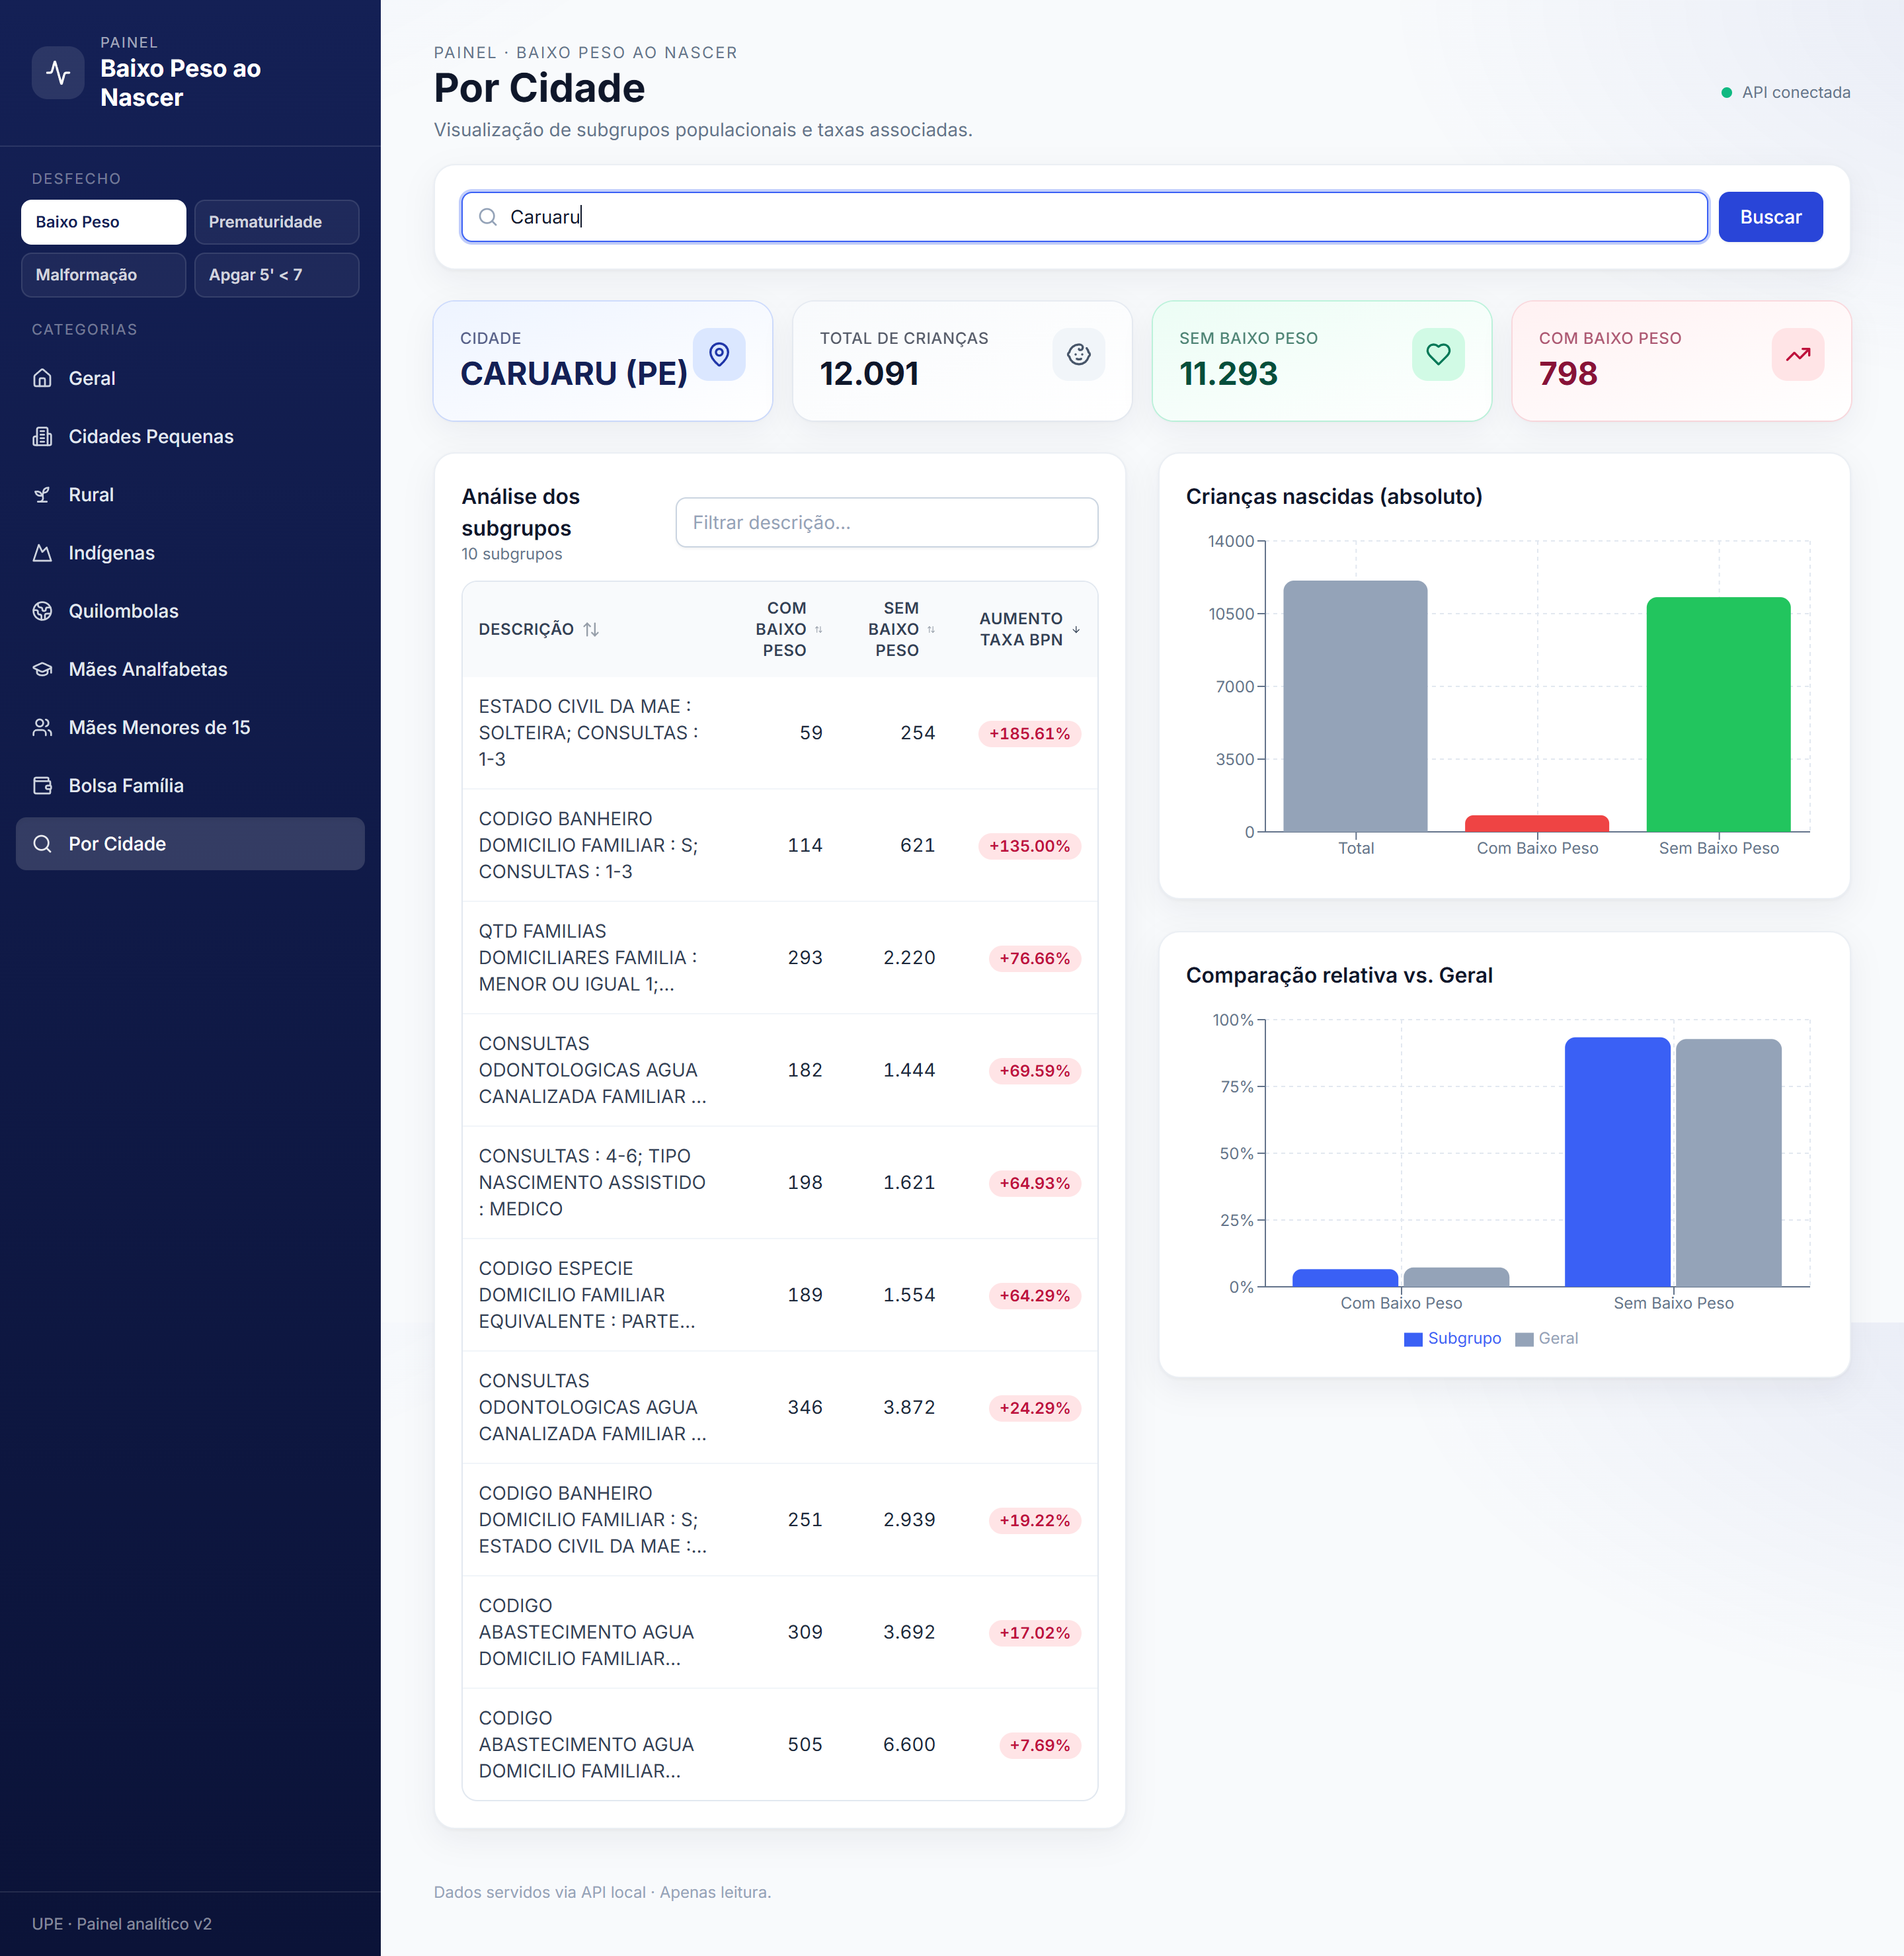
\includegraphics[width=\textwidth]{painel-caruaru}
\caption{Painel de visualização: subgrupos de malformação congênita no município de Caruaru (PE).}\label{fig:painel-caruaru}
\end{figure}

A navegação é feita por dois seletores, na barra lateral. O primeiro escolhe o desfecho (baixo peso, prematuridade, malformação ou Apgar no quinto minuto inferior a 7); o segundo escolhe a população, entre o recorte geral, os sete segmentos vulneráveis e a busca por município. Feita a escolha, o topo da tela resume a população selecionada em quatro indicadores: o nome do recorte, o total de nascimentos e quantos deles apresentaram ou não o desfecho. Em Caruaru, foram 12.091 nascimentos, dos quais 111 com malformação congênita, o que corresponde a uma prevalência basal de 0,92\%.

Abaixo dos indicadores, a tabela de análise lista os cinco subgrupos retornados para aquela população, numerados na ordem do SSDP+, da mesma forma que nas tabelas desta seção. Para cada regra, informa o número de nascimentos com e sem o desfecho e o aumento da taxa em relação à prevalência basal do recorte, que corresponde ao \emph{lift} menos um, expresso em porcentagem. A tabela pode ser ordenada por qualquer coluna e filtrada por texto, de modo que o usuário localize, por exemplo, todas as regras que envolvem o tipo de parto. Ao lado, um gráfico de barras mostra a prevalência do desfecho em cada subgrupo, com uma linha tracejada na prevalência basal do recorte: quanto mais a barra ultrapassa a linha, maior o \emph{lift} do subgrupo.

O exemplo de Caruaru reproduz, em escala municipal, o padrão observado na malformação congênita em todo o país, associado ao parto cesáreo, ao sexo masculino e a melhores condições de moradia. O parto cesáreo aparece em três das cinco regras (1, 4 e 5), o sexo masculino em outras três (1, 2 e 3), e itens como iluminação elétrica, domicílio de tijolo ou alvenaria e uma única família no domicílio se repetem entre elas. O subgrupo de maior risco (3) reúne ausência de calçamento, iluminação elétrica, domicílio de tijolo ou alvenaria, sexo masculino, uma única família no domicílio e despesas nulas com aluguel e medicamentos: são 2.053 nascimentos, 33 deles com malformação, o que equivale a uma prevalência de 1,61\%, 75\% acima da basal do município (\emph{lift} de 1,75). O subgrupo 1, com parto cesáreo e sexo masculino entre os seus itens, vem em seguida (71\% acima da basal), e a regra mais abrangente (4), com 6.347 nascimentos, combina parto cesáreo, uma única família no domicílio e despesa nula com transporte (22\% acima da basal). Assim, um gestor municipal pode identificar, em uma única consulta, os grupos em que a ocorrência do desfecho se concentra no seu território.

%% secoes/04-discussao.tex — incluído por main.tex

%%=====================================================================%%
\section{Discussão}\label{sec:discussao}
%%=====================================================================%%

Esta seção compara os quatro desfechos entre si, relaciona os resultados aos achados da literatura e apresenta as limitações do estudo.

%%---------------------------------------------------------------------%%
\subsection{Padrões comuns e específicos entre os desfechos}\label{subsec:disc-padroes}
%%---------------------------------------------------------------------%%

O número de consultas de pré-natal é o item que mais se repete entre os desfechos, mas com peso muito diferente em cada um. No baixo peso ao nascer, aparece em 23 dos 40 subgrupos e em todos os recortes; no nascimento pré-termo, está entre os cinco primeiros subgrupos dos oito recortes; no Apgar baixo, aparece em três recortes; e na malformação congênita não figura em nenhum subgrupo. Nos três desfechos em que aparece, a faixa de 1 a 3 consultas está associada aos maiores riscos: até 87\% acima da basal no baixo peso, até 103\% no pré-termo e até 86\% no Apgar baixo, quando isolada. A faixa de 4 a 6 consultas também eleva o risco, de 20\% a 46\% acima da basal no baixo peso e de 21\% a 46\% no pré-termo. Como as duas faixas correspondem às categorias do SINASC abaixo de sete ou mais consultas, o resultado indica que o risco permanece elevado mesmo quando o pré-natal foi iniciado, mas não completado.

A primeira gestação é o segundo item mais recorrente. No baixo peso, aparece em seis dos oito recortes e, combinada à faixa de 4 a 6 consultas, forma o subgrupo de maior risco nos municípios de até 10 mil habitantes, na população rural e na quilombola. No pré-termo, a mesma combinação eleva o risco em relação à faixa de 4 a 6 consultas isolada nos três recortes em que aparece, e no Apgar baixo a primeira gestação aparece combinada ao parto normal em três recortes, com risco entre 36\% e 40\% acima da basal.

Outros itens separam os desfechos. O sexo feminino acompanha o baixo peso, enquanto o sexo masculino aparece na malformação congênita, em todos os recortes, e no Apgar baixo, em seis deles. O parto cesáreo está presente nos oito recortes da malformação e no subgrupo de maior risco de seis deles, enquanto o parto normal aparece no Apgar baixo, em quatro recortes, e no baixo peso entre mães menores de 15 anos. Os itens de infraestrutura domiciliar também têm sentidos opostos: no baixo peso e na malformação, descrevem em sua maioria condições presentes, como banheiro, água canalizada e coleta de lixo; no Apgar baixo, descrevem condições ausentes ou precárias, como lixo não coletado, ausência de calçamento, domicílio improvisado e despesa total da família muito baixa.

Entre os segmentos, as mães menores de 15 anos concentram os valores mais altos: têm a maior prevalência basal de baixo peso (11,60\%), de pré-termo (17,26\%) e de malformação (0,63\%), e a segunda maior de Apgar baixo (3,13\%), além do subgrupo de maior risco do baixo peso (2,27 vezes a basal) e do subgrupo de maior risco do Apgar fora da população indígena (2,51 vezes). A população indígena apresenta o menor risco associado à faixa de 1 a 3 consultas, tanto no baixo peso quanto no pré-termo, e é o único segmento em que o nascimento domiciliar aparece como item de risco, no pré-termo (47\% acima da basal) e, sobretudo, no Apgar baixo, em que chega a 4,32 vezes a basal quando combinado a domicílio de 1 a 2 cômodos.

%%---------------------------------------------------------------------%%
\subsection{Relação com a literatura}\label{subsec:disc-literatura}
%%---------------------------------------------------------------------%%

Os itens mais recorrentes no baixo peso ao nascer coincidem com os fatores de maior risco identificados por regressão na mesma coorte: poucas consultas de pré-natal, primiparidade e sexo feminino \cite{falcao2020}. A diferença está no que cada abordagem retorna. A regressão estima o efeito de cada fator ajustado pelos demais; a descoberta de subgrupos mostra em quais combinações o desfecho se concentra e quanto cada combinação representa das ocorrências do segmento. O fato de cinco dos sete segmentos vulneráveis terem prevalência de baixo peso inferior à do recorte geral é compatível com o paradoxo epidemiológico do baixo peso ao nascer descrito para o Brasil, em que as maiores proporções se concentram nas áreas de maior desenvolvimento \cite{silva2010}, mas este estudo não permite separar esse efeito de diferenças de registro entre os segmentos.

No pré-termo, as maiores prevalências entre mães indígenas e mães muito jovens acompanham o padrão nacional descrito por estudos de séries temporais \cite{alberton2023,victor2025}, e o peso do número de consultas é coerente com o observado na Coorte de Nascimentos do CIDACS, em que poucas consultas se associaram tanto à prematuridade incidente quanto à recorrente \cite{rocha2022}. Naquele estudo, a idade materna de 14 a 19 anos e a raça/cor indígena se associaram apenas à prematuridade incidente, o que reforça que o peso de um mesmo atributo varia conforme o subconjunto analisado, como observado aqui entre os segmentos.

No Apgar baixo, os resultados se aproximam dos fatores maternos identificados em âmbito nacional, como menos de seis consultas, baixa escolaridade e raça/cor preta \cite{magalhaes2023}. O nascimento domiciliar entre indígenas, item de maior risco do desfecho, é coerente com o perfil descrito em território indígena do Pará, onde há gravidez na adolescência e baixa proporção de gestantes com sete ou mais consultas \cite{lima2025}. Já a maior prevalência basal entre mães menores de 15 anos difere do estudo nacional que deixou de encontrar a gravidez na adolescência como fator de risco em 2018--2019 \cite{magalhaes2023}; a diferença pode estar no recorte etário, mais restrito aqui, e no período analisado.

Na malformação congênita, os resultados se afastam da literatura. Estudos nacionais associam o desfecho à ausência de pré-natal e à raça/cor preta \cite{fernandes2025,trevilato2022}, enquanto aqui o número de consultas não aparece e os subgrupos de maior risco reúnem parto cesáreo, nascimento hospitalar e condições domiciliares presentes. Uma explicação possível é que esses itens indiquem maior chance de a anomalia ser detectada e registrada, e não maior ocorrência: a prevalência de anomalias no Brasil é considerada afetada pela detecção pré-natal e pela subnotificação, e a região de maior desenvolvimento apresenta as maiores taxas \cite{melkan2025}. Também é possível que o parto cesáreo seja consequência do diagnóstico pré-natal da anomalia, e não fator anterior a ela. Os dados disponíveis não permitem distinguir essas hipóteses.

%%---------------------------------------------------------------------%%
\subsection{Limitações}\label{subsec:disc-limitacoes}
%%---------------------------------------------------------------------%%

Os subgrupos descrevem associações, e não relações causais. Como cada regra é uma conjunção de itens, o risco de um subgrupo não isola o efeito de nenhum item individual, e a comparação entre regras só é direta quando elas diferem por um único item. Alguns atributos, como o tipo de parto e o local do nascimento, são registrados no momento do nascimento e podem ser consequência, e não antecedente, do desfecho ou da condição que o provocou. A WRAcc pondera a cobertura do subgrupo, o que favorece regras amplas, como as definidas apenas pelo sexo do recém-nascido, que aparecem entre as primeiras mesmo com risco baixo. Foram apresentados apenas os subgrupos da primeira execução do SSDP+, e alguns itens relevantes emergiram somente na segunda: no Apgar baixo da população indígena, por exemplo, o nascimento em local classificado como ``outros'' teve \emph{lift} de 6,43, ainda que com apenas 44 casos. Não foram calculados intervalos de confiança para o \emph{lift}.

Nos segmentos menores, as regras abrangem poucos casos, sobretudo na malformação congênita: os subgrupos de maior risco das populações quilombola e de mães menores de 15 anos reúnem 27 e 29 ocorrências, o que torna esses valores mais instáveis; o mesmo vale para os recortes municipais do painel. Algumas regras contêm itens redundantes em relação ao próprio segmento, como a idade materna inferior a 20 anos entre mães menores de 15 anos. Por fim, os dados referem-se a nascimentos de 2011 a 2015 em famílias de baixa renda registradas no Cadastro Único, o que limita a generalização para a população brasileira como um todo; dependem da qualidade de preenchimento do SINASC, em especial para as anomalias congênitas; e os atributos com muitos valores ausentes foram excluídos da formação das regras.

%% secoes/05-conclusao.tex — incluído por main.tex

%%=====================================================================%%
\section{Conclusão}\label{sec:conclusao}
%%=====================================================================%%

Este trabalho aplicou o algoritmo de descoberta de subgrupos SSDP+ a mais de 5 milhões de nascimentos da Coorte de 100 Milhões de Brasileiros vinculada ao SINASC, para quatro desfechos neonatais adversos e oito populações, em 32 análises independentes. 
A análise conjunta mostrou que alguns fatores se repetem entre os desfechos e outros são próprios de cada um. O número reduzido de consultas de pré-natal está associado aos maiores riscos de baixo peso ao nascer, nascimento pré-termo e Apgar baixo, e a primeira gestação acompanha esses três desfechos. A malformação congênita segue padrão distinto, com subgrupos marcados por parto cesáreo, sexo masculino e condições domiciliares presentes, o que sugere influência da detecção e do registro do desfecho.

A análise por segmento mostrou que os grupos vulneráveis não se comportam da mesma forma. As mães menores de 15 anos concentram as maiores prevalências e alguns dos maiores riscos relativos, enquanto na população indígena o nascimento domiciliar se destaca como item de risco para o pré-termo e para o Apgar baixo. Esses padrões não aparecem quando a população é analisada como um todo, o que justifica a análise separada de cada segmento. Os subgrupos encontrados foram disponibilizados em um painel interativo, que permite consultar e comparar os resultados por desfecho e por recorte.
O painel online também incluiu recortes por cidade com o objetivo de contribuir para a tomada de decisão no Brasil de forma mais capilarizada. 

Uma limitação importante deste trabalho é que os dados utilizados vão até 2015, o que pode reduzir a relevância para tomadas de decisões atuais.
Outra limitação é que o estudo não inclui relações de causa e efeito.
Como trabalhos futuros, propõe-se aplicar o método a dados mais recentes e investigar, com métodos adequados de inferência causal, associações relevantes deste estudo, como o papel do pré-natal incompleto e do nascimento domiciliar em populações indígenas.


%% Agradecimentos (opcional)
%% secoes/06-backmatter.tex — incluído por main.tex
%%
%% O template SBC não tem backmatter. A lista de abreviaturas e as
%% "Declarações" (financiamento, conflito de interesses etc.) eram
%% exigências da Springer Nature e foram retiradas. Se quiser
%% agradecimentos, descomente as linhas abaixo.

%% \section*{Agradecimentos}
%% Texto breve; números de auxílio ou de projeto podem ser mencionados aqui.


\bibliographystyle{sbc}
\bibliography{referencias/referencias}% arquivo .bib em referencias/

\end{document}
